\documentclass{rnu-thesis}

\usepackage[protrusion]{microtype}

% --- Algorithms (float + pseudocode)
\usepackage{algorithm}
\usepackage{algpseudocode}
\usepackage{float}
\usepackage{tikz}
\usetikzlibrary{positioning}
\usepackage{listings}
\usepackage{xcolor}

\usepackage{tikz} % harmless if already loaded via the class
\usetikzlibrary{arrows.meta,positioning,shapes.geometric,shapes.symbols,fit,calc,matrix,graphs}
\tikzset{>=Stealth}
\lstset{
    basicstyle=\ttfamily\small,
    breaklines=true,
    frame=single,
    numbers=left,
    numberstyle=\tiny,
    captionpos=b,
    showstringspaces=false
}

% % --- Code listings with minted (creates a 'listing' float)
% \usepackage[newfloat]{minted} % compile with -shell-escape
% --- Code listings without external deps

\lstset{
  basicstyle=\ttfamily\small,
  numbers=left,
  numbersep=6pt,
  frame=single,
  breaklines=true,
  tabsize=2,
  float=htbp, % keep if you want floaty listings
  captionpos=t % caption on top (to match your template)
}
% Optional: pick a mono font explicitly
% \setmonofont{Mono} % or Consolas/DejaVu Sans Mono/etc.


% --- Bibliography via biblatex ---
\usepackage[backend=biber,style=ieee,sorting=nty,maxbibnames=99]{biblatex}
\addbibresource{x_bibliography/references.bib}

% ====== Fill these in (example placeholders) ======
\setthesisinfoLV
  {Telegram Bot informācijas sistēmas izstrāde sabiedriskajam transportam Fergānas pilsētā}% LV Title
  {Rahimzhon Abdupaimov}% LV Student
  {Dr.sc.ing., Professor, Jelena Caiko}% LV Supervisor
  {42484 Informācijas sistēmas (bak.)}% LV Study programme
  {Dabaszinātņu un datortehnoloģiju katedra}% LV Department
  {2026}% Year

\setthesisinfoEN
  {Development of a Telegram Bot Information System for Public Transport in Fergana City}% EN Title
  {Rahimzhon Abdupaimov}% EN Student
  {Dr.sc.ing., Professor, Jelena Caiko}% EN Supervisor
  {42484 Information Systems (BSc)}% EN Study programme
  {Department of Natural Sciences and Computer Engineering}% EN Department
  {2026}% Year

% ====== MANUAL THESIS SCOPE - COUNT AND FILL IN MANUALLY ======
% Count your content manually and update these values:
% - Total pages: count final PDF pages
% - Tables/Figures/Algorithms/Listings: count from your List of Tables/Figures/etc.
% - Annexes: count appendix chapters after \appendix
% - References: count entries in your bibliography
\setthesisscope
  {52}% Total pages (count final PDF)
  {22}% Total tables (count from List of Tables)
  {8}% Total figures (count from List of Figures) 
  {0}% Total algorithms (count from List of Algorithms)
  {6}% Total listings (count from List of Listings)
  {2}% Total annexes (count appendix chapters)
  {18}% Total references (count bibliography entries)

\begin{document}

\input{a_frontmatter/title_page_lv}
\clearpage
\input{a_frontmatter/title_page_en}
\clearpage

% Page numbering starts at Title page but number not printed there (done).
% Show numbers from here:
\pagenumbering{arabic}

% ===== Abstracts & Keywords =====
\section*{Anotācija}
\addcontentsline{toc}{section}{Anotācija (LV)}

\textbf{Nosaukums:} Telegram Bot informācijas sistēmas izstrāde
sabiedriskajam transportam Fergānas pilsētā.

\medskip

Sabiedriskajam transportam Fergānā -- aptuveni 300\,000 iedzīvotāju
lielā pilsētā Uzbekistānā -- nav oficiālas digitālās informācijas
sistēmas. Iedzīvotāji un viesi paļaujas uz mutisku informāciju, papīra
zīmēm vai vispārīgiem karšu pakalpojumiem, piemēram, Yandex Maps, kas
nesniedz pilnīgus datus par vietējiem autobusu maršrutiem. Tas rada
ikdienas problēmas: cilvēki nokavē autobusus, izvēlas nepareizus
maršrutus vai pavada lieku laiku pieturās.

Darba mērķis ir izstrādāt Telegram bota informācijas sistēmu, kas
vienkāršā un pieejamā veidā nodrošina sabiedriskā transporta
informāciju Fergānas pilsētā. Telegram tika izvēlēts tāpēc, ka tas ir
viens no populārākajiem ziņojumapmaiņas lietotnēm Uzbekistānā un labi
darbojas pat uz lētiem viedtālruņiem ar ierobežotu internetu.

Bots tika izstrādāts valodā Python, izmantojot \texttt{aiogram}
ietvaru un SQLite datubāzi. Maršrutu un pieturu dati tika apkopoti no
Yandex Maps un saglabāti vietējā datubāzē. Bots atbalsta sešus
autobusu maršrutus un piedāvā šādas galvenās funkcijas: maršruta
pieturu rādīšanu, maršruta meklēšanu starp divām pieturām, taksometru
informāciju un lietotāju ieteikumu vākšanu. Sistēma tika izvietota
PythonAnywhere mākoņa platformā nepārtrauktai darbībai.

Bots tika testēts ar nelielu lietotāju grupu Fergānā. Rezultāti rāda,
ka sistēma ir viegli lietojama, ātri reaģē un aptver biežākos
transporta jautājumus. Darbā arī tiek aplūkoti turpmākie uzlabojumi,
tostarp integrācija ar Grok AI modeli dabiskās valodas vaicājumiem.

Darbs apstiprina, ka Telegram bots ir praktisks un zemu izmaksu
risinājums pilsētām, kurās nav oficiālu transporta lietotņu.

\medskip

\noindent\textbf{Apjoms:} XX lappuses, YY tabulas, ZZ attēli,
zx atsauces, xz pielikumi.
\newpage

\section*{Abstract}
\addcontentsline{toc}{section}{Abstract (EN)}

\textbf{Title:} Development of a Telegram Bot Information System for
Public Transport in Fergana City.

\medskip

Public transport in Fergana, a city of about 300{,}000 inhabitants in
Uzbekistan, has no official digital information system. Residents and
visitors depend on word of mouth, paper signs, or general map services
such as Yandex Maps, which do not provide full data on local bus routes.
This creates daily problems: people miss buses, take wrong routes, or
spend extra time at stops.

The aim of the thesis is to design and develop a Telegram bot
information system that provides public transport information for
Fergana city in a simple and accessible way. Telegram was chosen because
it is one of the most popular messengers in Uzbekistan and works well
on low-end smartphones with limited internet.

The bot was developed in Python using the \texttt{aiogram} framework
and SQLite as the database. Route and stop data were collected from
Yandex Maps and stored in a local database. The bot supports six bus
routes and the following main functions: showing route stops, searching
a route between two stops, providing taxi information, and collecting
user suggestions. The system was deployed on the PythonAnywhere cloud
platform for continuous operation.

The bot was tested with a small group of users in Fergana. Results show
that the system is easy to use, responds quickly, and covers the most
common transport questions. The thesis also discusses future
improvements, including integration with the Grok AI model for natural
language queries.

The work confirms that a Telegram bot is a practical and low-cost
solution for cities where official transport applications do not exist.

\medskip

\noindent\textbf{Volume:} XX pages, YY tables, ZZ figures,
zx references, xz appendices.
\newpage

\section*{Keywords}
\addcontentsline{toc}{section}{Keywords}

Telegram bot; public transport; urban mobility; information system;
Fergana; Uzbekistan; chatbot; Python; aiogram; SQLite; transport
informatization; messenger-based services; route search; user-centered
design.

\vspace{1em}

\noindent\textbf{Atslēgvārdi (LV):} Telegram bots; sabiedriskais transports;
pilsētas mobilitāte; informācijas sistēma; Fergāna; Uzbekistāna; tērzēšanas
bots; Python; aiogram; SQLite; transporta informatizācija; uz ziņojumapmaiņu
balstīti pakalpojumi; maršrutu meklēšana; lietotājorientēts dizains.
\newpage


% ===== Table of Contents (and optional lists) =====
\tableofcontents

% ---- Meta lists: each on its own page, and not added to ToC ----
\clearpage
\begingroup\let\addcontentsline\relax\listoffigures\endgroup

\clearpage
\begingroup\let\addcontentsline\relax\listoftables\endgroup

\clearpage
\begingroup\let\addcontentsline\relax\listofalgorithms\endgroup

\clearpage
% \begingroup\let\addcontentsline\relax\listoflistings\endgroup
\begingroup\let\addcontentsline\relax\lstlistoflistings\endgroup
\clearpage



% ===== Chapters =====
% Unnumbered Introduction (still added to ToC)
\unchapter{Introduction}

Public transport is an important part of daily life in every city. Many people use buses, minibuses, and taxis to go to work, school, university, markets, hospitals, and other places. For this reason, clear transport information is very important. A person needs to know which route to take, where the stop is, and how to reach the needed place.

Fergana is one of the important cities of Uzbekistan. \cite{stat_uz_fergana} It is a regional city with many residents, students, workers, and visitors. Public transport in Fergana is used every day. Minibuses and buses are common means of transport. Taxi services are also widely used. However, transport information is often not collected in one digital system. A user may need to ask other people, search in social networks, or learn routes by personal experience. This is not always fast and comfortable.

The problem is especially important for new residents, students, tourists, and people who do not know the city well. They may not know which route goes to a needed place. They may also not know the names of stops. In many cases, the information is available only from local people. This creates a practical problem. The user does not have one simple and free source of transport information.

Today, many people in Uzbekistan use Telegram. \cite{datareportal_uz_2024} Telegram is a messaging application. A messaging application is a program for sending and receiving messages. Telegram also supports bots. A bot is a small program that works inside Telegram and answers user commands. A Telegram bot can give information automatically. The user does not need to install a new mobile application. The user only needs Telegram, which is already installed on many phones.

For this reason, a Telegram bot can be a suitable solution for public transport information in Fergana. It can work at any time. It can be free for users. It can store route data in a database. A database is a structured place for storing information. In this work, the database stores routes, stops, taxi services, and user records for simple analytics.

The developed system is called \textbf{Fergana Transport Bot}. The bot is designed as a simple information system. An information system is a system that collects, stores, processes, and gives information to users. In this project, the system gives public transport information to Telegram users. The main users are residents and visitors of Fergana city.

\textbf{Topicality of the problem.}

The topic is relevant because Fergana city does not have a centralized, free, and easy-to-use digital information system for public transport. Public transport users often need quick information about routes and stops. If this information is not easy to find, users lose time. They may choose the wrong route. They may need to ask other people. This is not convenient.

Digital services can help to solve this problem. A mobile application is one possible solution. However, a mobile application needs installation. It also needs more development time and more support. In the scope of this bachelor thesis, Telegram is a more practical choice. Telegram is already popular in Uzbekistan. A Telegram bot is easy to open and easy to use. It can work on different devices. It can work on phones and computers.

The topic also has practical value. The system can help people find transport information faster. It can also be extended in the future. For example, it can be used in other regional cities of Uzbekistan. It can also be improved with an admin panel, maps, or artificial intelligence in the future. Artificial intelligence is not included in the current version. It is moved to future development to keep the project focused.

The topic is also suitable for an Information Systems bachelor thesis. It includes problem analysis, system design, database design, software development, testing, and evaluation. These parts match the study programme of Information Systems.

\textbf{Aim of the study.}

The aim of the study is to develop a Telegram bot information system that helps Fergana residents and visitors find information about public transport routes, stops, and taxi services.

\textbf{Object of the study.}

The object of the study is the information support of public transport users in regional cities of Uzbekistan.

\textbf{Subject of the study.}

The subject of the study is the development of a Telegram bot as an information system for public transport in Fergana city.

\textbf{Research problem.}

The research problem is that Fergana has no centralized, free, and easy-to-use digital information system for public transport. As a result, users do not always have fast access to route, stop, and taxi information.

The problem can be described in the following way. Public transport information exists in the city, but it is not always organized in one place. Some users know routes from personal experience. Some users ask other people. Some users search in social networks. These ways are not stable and not always correct. A simple digital system can reduce this problem.

\textbf{Tasks of the study.}

To achieve the aim of the study, the following tasks are defined:

\begin{enumerate}
    \item To review literature about information systems, public transport information services, Telegram bots, and database systems.
    \item To analyze the current situation of public transport information in Fergana city.
    \item To design the structure of the Telegram bot and the SQLite database.
    \item To develop the Telegram bot using Python and the aiogram library.
    \item To add real transport data about routes, stops, and taxi services to the database.
    \item To test the bot with a small group of users and evaluate the results.
    \item To prepare proposals for future improvement of the system.
\end{enumerate}

\textbf{Hypothesis.}

The hypothesis of the study is that a Telegram bot connected to a SQLite database can give Fergana residents fast and reliable access to transport information. It can be more accessible than a mobile application because Telegram is already installed on many users' phones.

\textbf{Research methods.}

Several research methods are used in this thesis.

The first method is literature analysis. Literature analysis means reading and studying books, articles, documentation, and online sources. This method is used to understand information systems, Telegram bots, databases, and public transport information systems.

The second method is case analysis. Case analysis means studying one real situation. In this thesis, the case is public transport information in Fergana city. This method helps to understand the local problem and user needs.

The third method is system design. System design means planning how the system will work before coding. In this work, system design includes bot commands, database tables, and the general architecture of the system.

The fourth method is software development. Software development means creating a working program. In this thesis, the bot is developed in Python. Python is a programming language. The bot uses aiogram. Aiogram is a Python library for Telegram bots. A library is ready-made code that helps developers build software faster.

The fifth method is database modelling. Database modelling means planning how data will be stored. In this work, SQLite is used. SQLite is a small database system. It stores data in one file. This is enough for a small public transport information system.

The sixth method is testing. Testing means checking if the system works correctly. The bot is tested with main commands. These commands include route search, stop information, taxi information, and help information.

The seventh method is user feedback. User feedback means collecting opinions from real users. In this thesis, the system is tested in a small pilot test with users from the student's personal network in Fergana. A pilot test is a small first test of a system.

\textbf{Description of the developed system.}

The developed system is a Telegram bot named \textbf{Fergana Transport Bot}. It uses Python as the main programming language. It uses the aiogram library to communicate with Telegram. It uses SQLite as the database. The bot stores and shows information about routes, stops, and taxi services.

The main commands of the bot are:

\begin{itemize}
    \item \texttt{/start} -- shows a welcome message and main information;
    \item \texttt{/help} -- shows all available commands;
    \item \texttt{/marshrut <number>} -- shows stops for a selected route;
    \item \texttt{/poisk <from> <to>} -- searches for a route between two stops;
    \item \texttt{/taxi} -- shows taxi services and phone numbers;
    \item \texttt{/dobavit} -- allows users to suggest new transport information.
\end{itemize}

The database has five main tables. These tables are routes, stops, route stops, taxi services, and users. The routes table stores route numbers and descriptions. The stops table stores stop names. The route stops table connects routes with stops. The taxi services table stores taxi names and phone numbers. The users table stores Telegram user identifiers for simple analytics.

The system is developed as a minimum viable product. A minimum viable product, or MVP, is the first working version of a system. It includes the most important functions. In the scope of this bachelor thesis, the MVP approach is suitable because the goal is to build a working and testable system, not a large commercial platform.

\textbf{Practical value of the study.}

The practical value of this work is that the system can help public transport users in Fergana city. A user can open Telegram and send a command to the bot. The bot can answer with route, stop, or taxi information. This can save time for users.

The system is also useful because it is low-cost. It does not need a separate mobile application. It does not need a complex database server. SQLite was chosen because the data volume is small and a separate database server is not needed. The bot can be hosted on a low-cost or free hosting service. This is important for a student project and for possible local use.

The architecture also allows future improvement. The system can later include more routes, more stops, maps, an admin panel, and artificial intelligence. However, these functions are not part of the current implementation. They are discussed as future work.

\textbf{Approbation of the study.}

The results of the study were tested in a small pilot test with users from the student's personal network in Fergana. The users checked the main bot commands and gave simple feedback about usability and usefulness. The results of this test are used in Chapter 3 of the thesis.

The work can also be presented during the bachelor thesis defence at Riga Nordic University. The defence will include the problem, aim, developed system, database structure, testing results, and future improvements.

\textbf{Defended thesis.}

The following defended thesis statements are proposed:

\begin{enumerate}
    \item Has been offered a new Telegram bot system for public transport information in Fergana city, based on Python and SQLite.
    \item Has been modified the traditional approach of accessing transport information by moving it from offline sources to a 24/7 digital channel inside Telegram.
    \item Has been suggested an extensible architecture that allows future integration with AI assistants for handling free-form questions.
\end{enumerate}

\textbf{Structure of the thesis.}

The thesis consists of an introduction, four main chapters, conclusions, literature, and appendices.

The introduction explains the topicality of the problem, aim, object, subject, research problem, tasks, hypothesis, methods, approbation, and defended thesis.

Chapter 1 presents the literature review and theoretical background. It explains key concepts, related work, theoretical ideas, and the motivation for the chosen direction.

Chapter 2 presents the case and system analysis. It describes the situation in Fergana city, the environment of the system, constraints, risks, and data collection methods.

Chapter 3 presents the practical research. It describes the design and development of the Telegram bot, database structure, commands, screenshots, testing results, and evaluation.

Chapter 4 discusses the results and future development. It presents possible improvements, feasibility, efficiency, and further development directions.

Chapter 5 presents the conclusions. It explains how the aim was achieved, how the tasks were completed, and how the hypothesis was checked.
\clearpage
\chapter{Literature Review and Theoretical Background}
\label{chap:litreview}
\label{ch:literature}

\section{Core Concepts and Definitions}
\label{sec:concepts}

Before discussing the system design and the implementation, it is important to explain the main concepts used in this thesis. These concepts form the basic theoretical background of the work. They help to describe the problem clearly and to show why a Telegram bot is a suitable solution for public transport information in Fergana city.

An \textbf{information system} is a system that collects, stores, processes, and provides information to users. In simple words, it helps people find the information they need in a structured way. In this thesis, the developed system is an information system because it stores transport data and gives it to users through Telegram.

A \textbf{Telegram bot} is a program that works inside Telegram and responds to user commands. A bot can send messages automatically, answer questions, and show stored information. Telegram bots are useful because they are easy to access and do not require installation of a separate mobile application.\cite{telegram_botapi}

A \textbf{database} is a structured place for storing information. It keeps data in an organized form so that it can be searched, updated, and used by a program. In this thesis, the database stores routes, stops, taxi services, and user records. \cite{elmasri2016database}

\textbf{SQLite} is a lightweight database system. It stores data in one local file and does not need a separate database server. SQLite is suitable for small and medium projects, especially when the system needs to be simple, reliable, and easy to deploy.\cite{sqlite_docs, kreibich2010sqlite}

A \textbf{route} is the path that a bus, minibus, or taxi follows from one point to another. A \textbf{stop} is a place where passengers get on or off public transport. These two concepts are important because the main goal of the bot is to help users find route and stop information quickly.

A \textbf{taxi service} is a transport service that carries passengers by car. In this thesis, taxi services are included because many people in Fergana use both public transport and taxis in daily life. For this reason, the bot does not only show bus and minibus routes, but also gives useful taxi information.

A \textbf{user} is a person who interacts with the system. In this project, the users are residents of Fergana, students, visitors, and other people who need transport information. The system is designed to be simple enough for all these groups.

A \textbf{minimum viable product (MVP)} is the first working version of a system that contains only the most important functions. MVP is often used in student and startup projects because it allows the developer to test the main idea first and improve the system later. In this thesis, the Telegram bot is developed as an MVP. \cite{sommerville2016software}

Table~\ref{tab:core_concepts} summarizes the main terms used in the thesis.

\begin{table}[H]
\centering
\caption{Main concepts used in the thesis}
\label{tab:core_concepts}
\begin{tabular}{|p{4cm}|p{5cm}|p{5cm}|}
\hline
\textbf{Concept} & \textbf{Simple definition} & \textbf{Role in this thesis} \\
\hline
Information system & A system that collects, stores, processes, and provides information & The developed bot works as an information system for transport data \\
\hline
Telegram bot & A program inside Telegram that answers user commands automatically & The main interface of the project \\
\hline
Database & A structured place for storing data & Stores routes, stops, taxi services, and users \\
\hline
SQLite & A lightweight database system stored in one file & Used as the database technology in the project \\
\hline
Route & The path followed by public transport & One of the main data types shown by the bot \\
\hline
Stop & A place where passengers enter or leave transport & Used for route search and route description \\
\hline
Taxi service & A car-based passenger transport service & Included as additional useful transport information \\
\hline
MVP & The first working version of a system with key functions & Describes the implementation strategy of the project \\
\hline
\end{tabular}
\end{table}

These definitions show that the project combines transport information, database storage, and Telegram-based interaction. This combination is simple, practical, and suitable for users who need fast access to transport data. The next sections will discuss related work and theoretical ideas in more detail.

\section{Related Work: Themes, Methods, Evidence}
\label{sec:related}

Public transport information systems are widely used in many cities. Their main purpose is to help passengers understand how to move from one place to another. Such systems can show routes, stops, timetables, vehicle locations, ticket information, and other useful data. In large cities, these systems are often connected with official transport operators and map services. In smaller or regional cities, such systems may be less developed or not available in a simple digital form. \cite{kasinathan2020transport}

Modern transport information services can be divided into several groups. The first group includes official mobile applications. These applications are usually developed by city transport departments or private companies. They may include route maps, timetables, and real-time vehicle tracking. The second group includes web services. These services work through a browser and can be used on phones and computers. The third group includes map platforms such as Google Maps or Yandex Maps. They can provide navigation and route suggestions in some cities. The fourth group includes messaging bots, including Telegram bots. These bots give information through a chat interface.\cite{adamopoulou2020chatbots, dale2016return}

Each solution has advantages and limitations. A mobile application can have many functions, but it requires installation. It also needs regular updates and support for different devices. A website is easier to access, but it may not be as convenient as a chat interface for quick questions. Map platforms are powerful, but they do not always contain complete local route information for smaller cities. A Telegram bot is simpler, but it can be very practical if users already use Telegram every day. \cite{following2019messaging}

Table~\ref{tab:transport_tools_comparison} compares different types of public transport information tools.

\begin{table}[H]
\centering
\caption{Comparison of public transport information tools}
\label{tab:transport_tools_comparison}
\begin{tabular}{|p{3.2cm}|p{4cm}|p{3.5cm}|p{3.5cm}|}
\hline
\textbf{Tool type} & \textbf{Main advantages} & \textbf{Main limitations} & \textbf{Suitability for this project} \\
\hline
Mobile application & Can include maps, notifications, and many functions & Requires installation and more development time & Less suitable for MVP because it is more complex \\
\hline
Website & Can be opened in a browser and updated centrally & May be less convenient for quick chat-based use & Possible, but not the main choice \\
\hline
Map platform & Provides navigation and visual maps & Local route data may be incomplete or unavailable & Useful as support, but not enough as the main system \\
\hline
Telegram bot & Easy to access, works inside a popular messenger, does not require a new app & Limited interface compared to a full mobile app & Highly suitable for a simple transport information MVP \\
\hline
\end{tabular}
\end{table}

The comparison shows that a Telegram bot is a practical solution for the scope of this bachelor thesis. It is not the most complex tool, but it is accessible and easy to use. This is important because the goal of the project is not to create a large commercial platform, but to develop a working information system for public transport data in Fergana city.

Several themes are important in related work on digital transport information systems. The first theme is accessibility. A transport information system should be easy to access for different groups of users. These users may include students, workers, older people, tourists, and new residents. If the system is difficult to install or use, many people will not use it.

The second theme is data organization. Transport information must be stored in a structured way. Routes, stops, and services should not be stored only as plain text. They should be placed in a database so that the system can search and show them correctly. A database also makes future improvement easier.

The third theme is user interaction. A good transport information system should allow users to ask for information quickly. In the case of a Telegram bot, this interaction is based on commands and messages. The user can type a command such as \texttt{/marshrut 10} or \texttt{/taxi}, and the bot returns the needed information.

The fourth theme is maintainability. A digital system should be easy to update. Public transport data can change. New stops may appear. Route names and taxi phone numbers may be updated. For this reason, the system architecture should allow future changes.

Table~\ref{tab:related_work_themes} summarizes the main themes that are important for this project.

\begin{table}[H]
\centering
\caption{Main themes from related work}
\label{tab:related_work_themes}
\begin{tabular}{|p{4cm}|p{6cm}|p{4cm}|}
\hline
\textbf{Theme} & \textbf{Meaning} & \textbf{Application in this thesis} \\
\hline
Accessibility & The system should be easy to open and use & Telegram is used because many users already have it \\
\hline
Data organization & Transport data should be stored in a structured form & SQLite database stores routes, stops, taxi services, and users \\
\hline
User interaction & Users should receive answers quickly and clearly & Bot commands are used for simple interaction \\
\hline
Maintainability & The system should be easy to update and extend & The database structure supports adding new routes and stops \\
\hline
Scalability & The system should allow future growth & Future versions may include maps, admin panel, and AI support \\
\hline
\end{tabular}
\end{table}

For this thesis, related work supports the idea that a simple digital transport information system can be useful even without advanced functions. The most important point is that users must have one clear place where they can find route and stop information. A Telegram bot can provide this function in a practical way. \cite{kamberi2021telegram}\cite{shawar2007chatbots}


\section{Theoretical Framework}
\label{sec:framework}

The Fergana Transport Bot is designed as an information system with five
main parts: the user, the messaging client (Telegram), the bot
application, the database, and the hosting environment. These parts work
together in a client--server architecture with asynchronous message
passing. This framework is widely used in modern chat bots because it can
handle many user requests at the same time without blocking the server.

The general flow of a user request is shown in
Figure~\ref{fig:framework}. The user sends a command from the Telegram
client. The Telegram servers forward the command to the bot through the
Bot API. The bot application processes the command, reads data from the
database, and sends the answer back to the user through the same
channel.

\begin{figure}[h]
\centering
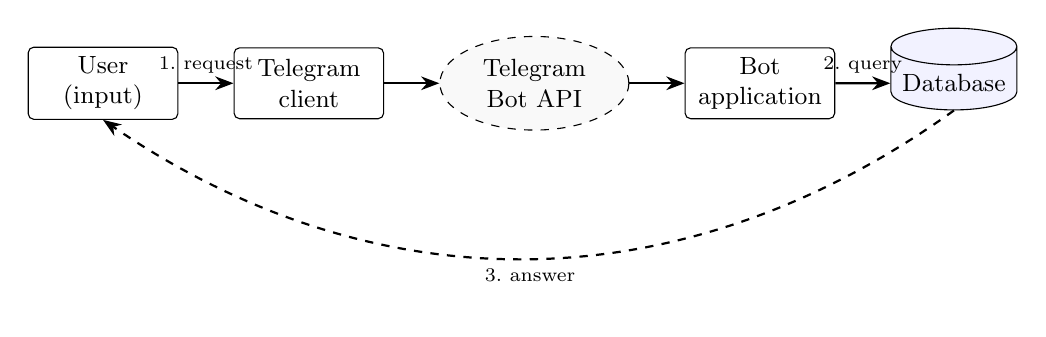
\begin{tikzpicture}[
    node distance=1.0cm and 0.7cm,
    box/.style={rectangle, draw, rounded corners=2pt, minimum width=1.9cm,
        minimum height=0.9cm, align=center, font=\small},
    db/.style={cylinder, draw, shape border rotate=90, aspect=0.3,
        minimum width=1.6cm, minimum height=0.9cm, align=center,
        font=\small, fill=blue!5},
    cloud/.style={ellipse, draw, dashed, minimum width=2.4cm,
        minimum height=1.0cm, align=center, font=\small, fill=gray!5},
    arrow/.style={->, >=Stealth, thick}
]
    \node[box] (user) {User\\(input)};
    \node[box, right=of user] (tg) {Telegram\\client};
    \node[cloud, right=of tg] (api) {Telegram\\Bot API};
    \node[box, right=of api] (bot) {Bot\\application};
    \node[db, right=of bot] (db) {Database};

    \draw[arrow] (user) -- node[above, font=\scriptsize] {1.~request} (tg);
    \draw[arrow] (tg) -- (api);
    \draw[arrow] (api) -- (bot);
    \draw[arrow] (bot) -- node[above, font=\scriptsize] {2.~query} (db);
    \draw[arrow, dashed] (db.south) to[bend left=35]
        node[below, font=\scriptsize] {3.~answer} (user.south);
\end{tikzpicture}
\caption{Theoretical framework: client--server flow of a bot request}
\label{fig:framework}
\end{figure}

The framework can also be described with the classic
\textit{input--processing--output} model. The input is the user message.
The processing is the matching of the message to a command handler and
the database query. The output is the reply text sent back to Telegram.
This simple model is enough for a small public transport information
system and matches well with the asynchronous programming style of the
aiogram library. \cite{aiogram_docs}

Three properties of this framework are important for the project:

\begin{itemize}
    \item \textbf{Statelessness of the API.} Each request is independent.
        The bot does not need to keep a long session for every user.
    \item \textbf{Asynchronous processing.} Many requests can be handled
        in parallel. The waiting time for one user does not block
        another.\cite{python_asyncio}
    \item \textbf{Separation of data and code.} Routes, stops, and taxi
        services live in the database. The Python code only handles
        commands and formatting. New data can be added without changing
        the code.
\end{itemize}

These three properties shape the design decisions in
Chapter~\ref{ch:development}. They explain why aiogram, SQLite, and a
modular command-handler structure are a good fit for the Fergana
Transport Bot.

\section{Illustrative Code Snippet}
\label{sec:code-snippet}

To make the theoretical framework concrete, this section presents a
small code example. Listing~\ref{lst:framework-handler} shows the
typical structure of an aiogram command handler. The example
demonstrates how the input--processing--output model from
Section~\ref{sec:framework} is implemented in Python. \cite{aiogram_docs}

\begin{lstlisting}[language=Python, caption={Example of an asynchronous
    command handler in aiogram}, label={lst:framework-handler}]
from aiogram import Dispatcher, types
from aiogram.filters import Command

dp = Dispatcher()

@dp.message(Command("marshrut"))
async def handle_route_command(message: types.Message):
    # 1. INPUT: read the command argument from the user message
    args = message.text.split(maxsplit=1)
    if len(args) < 2:
        await message.answer("Please enter a route number.")
        return
    route_number = args[1].strip()

    # 2. PROCESSING: read the matching data from the database
    stops = db.get_stops_by_route(route_number)

    # 3. OUTPUT: send the formatted answer back to the user
    if not stops:
        await message.answer(f"Route {route_number} not found.")
    else:
        text = f"Route {route_number}:\n" + "\n".join(stops)
        await message.answer(text)
\end{lstlisting}

The example shows three important features that are typical for the
chosen framework. First, the function is declared with the
\texttt{async} keyword. This means many users can call the handler at
the same time without blocking the server. Second, the
\texttt{@dp.message(Command("marshrut"))} decorator links the handler
to a specific command. The same pattern is used for every command in
Chapter~\ref{ch:development}. Third, the database call and the answer
sending are clearly separated. This separation makes the code easy to
read, easy to test, and easy to extend with new commands.

\section{Research Motivation and Direction}
\label{sec:motivation}

This section explains why the project is worth doing, what gap it fills,
and what its scope is. The motivation is based on the problem statement
in the Introduction, the concepts in Section~\ref{sec:concepts}, and
the comparison with related work in Section~\ref{sec:related}.

\subsection{Significance of the Problem}
\label{subsec:significance}

Fergana is a regional capital with about 300\,000 inhabitants. Daily
mobility in the city depends on public buses, shared minibuses, and
taxis. Despite this, the city has no centralized digital information
system for public transport. Residents and visitors lose time every day
because they cannot quickly find the right route or stop. The problem
affects students, workers, older residents, and tourists. A simple and
free digital tool can reduce this daily loss of time.\cite{stat_uz_fergana}

\subsection{Identified Gap}
\label{subsec:gap}

The related work analysis in Section~\ref{sec:related} showed that
similar transport information bots exist for larger cities such as
Moscow and Tashkent. However, no such bot exists for Fergana. General
map platforms such as Yandex Maps cover only a part of the local routes.
A summary of the gap is shown in Table~\ref{tab:gap}.

\begin{table}[h]
\centering
\caption{Gap analysis: existing solutions vs. needs of Fergana}
\label{tab:gap}
\begin{tabular}{p{0.32\textwidth}p{0.30\textwidth}p{0.30\textwidth}}
\hline
\textbf{Need of Fergana users} & \textbf{Existing solutions} &
\textbf{Gap} \\
\hline
Quick access without
installation & Mobile apps require install & No bot for Fergana \\
Full coverage of local
bus routes & Yandex Maps covers part of routes & Local routes missing \\
Free and zero-cost service
& Some commercial apps & No free local tool \\
Familiar interface for
local users & Telegram is widely used & Not used yet for this task \\
Easy update of route data
& Closed databases of operators & No open editable dataset \\
\hline
\end{tabular}
\end{table}

The gap is clear: Fergana users have a real need, but no existing tool
covers it fully. A Telegram bot connected to a local database can fill
this gap with low cost and low technical risk.

\subsection{Direction and Scope}
\label{subsec:scope}

Based on the identified gap and the chosen framework, the direction of
the project is set as follows. The thesis develops a Telegram bot with a
manually curated SQLite database for Fergana minibuses, bus stops, and
taxi services. The bot is implemented in Python with the aiogram
library and deployed on a free cloud platform. The project is built as
a minimum viable product (MVP). It focuses on the most important
functions: showing route stops, searching a route between two stops,
and providing taxi contacts.

The scope of the thesis is limited on purpose. The following items are
\textbf{out of scope} for the current work:

\begin{itemize}
    \item GPS-based real-time tracking of vehicles, because no public
        GPS data is available in Fergana.
    \item Integration with payment systems for tickets, because there
        is no electronic ticket system in the city.
    \item A separate native mobile application, because the main idea
        of the project is that Telegram is enough.
    \item Free-form AI question answering, because it adds external
        dependencies and is better suited as future work.
\end{itemize}

These items are not ignored. They are discussed in
Chapter~\ref{ch:discussion} as proposals for future development.

\subsection{Success Criteria}
\label{subsec:success}

The success of the project is measured by clear criteria. These
criteria are used later in Chapter~\ref{ch:development} to evaluate the
final bot. The criteria are shown in Table~\ref{tab:success-criteria}.

\begin{table}[h]
\centering
\caption{Success criteria of the project}
\label{tab:success-criteria}
\begin{tabular}{lp{0.5\textwidth}}
\hline
\textbf{Criterion} & \textbf{Target} \\
\hline
Response time & Average reply time below 2 seconds. \\
Coverage & At least five Fergana bus routes in the database. \\
Reliability & Success rate of common requests above 90\,\%. \\
User feedback & Positive feedback from more than 70\,\% of test users. \\
Availability & The bot is hosted 24/7 on a free cloud platform. \\
\hline
\end{tabular}
\end{table}

These criteria are realistic for a bachelor thesis. They are also
strict enough to show whether the chosen direction works in practice.

\section{Chapter Summary}
\label{sec:ch1-summary}

This chapter presented the theoretical background of the thesis. The
main concepts used in the work were defined in Section~\ref{sec:concepts}:
information system, Telegram bot, database, SQLite, route, stop, taxi
service, user, and minimum viable product. These concepts form the
common vocabulary used in the rest of the thesis.

Section~\ref{sec:related} reviewed related work and compared four types
of transport information tools: mobile applications, websites, map
platforms, and messaging bots. The comparison showed that a Telegram
bot is a suitable solution for the specific context of Fergana city,
where users already use Telegram every day and where general map
platforms do not provide full route coverage.

Section~\ref{sec:framework} described the theoretical framework of the
project as a client--server system with asynchronous message passing.
The input--processing--output model was used to explain how a user
request becomes an answer. The framework was made concrete in
Section~\ref{sec:code-snippet} with an example aiogram handler that
follows the same model in Python code.

Section~\ref{sec:motivation} explained the significance of the problem,
described the gap left by existing solutions, set the scope of the
work, and listed five success criteria. The criteria will be used in
Chapter~\ref{ch:development} to evaluate the final system.

These choices motivate the case and system analysis presented in the
next chapter. Chapter~\ref{ch:analysis} describes the city of Fergana,
the local transport context, user groups, and the functional and
non-functional requirements of the system.
\chapter{Case Analysis: Public Transport in Fergana City}
\label{ch:case}
\label{ch:analysis}

This chapter analyses the case city of the thesis. It describes the
city of Fergana, its public transport system, the main problems faced
by passengers, and the requirements for a digital information service.
The chapter creates the practical context for the system that is
designed and built in Chapter~\ref{ch:empirical}.

\section{City Profile and Transport Context}
\label{sec:city-profile}

Fergana is a regional capital in the east of Uzbekistan with a
population of approximately 300{,}000 people \cite{stat_uz_fergana}.
The city is the administrative and economic centre of the Fergana
Valley, one of the most densely populated regions in Central Asia. Daily
mobility in the city depends mostly on public buses and shared taxis.
Private cars are common but not the main mode of transport for
students, pensioners, and low-income groups.

Public bus transport in Fergana is operated by several local carriers.
There is no single official operator that publishes a complete schedule
or a digital map of routes. Information about routes is shared mostly
through signs on buses, word of mouth, and unofficial posts in social
networks. General map services such as Yandex Maps cover only a part of
the local routes and do not provide reliable real-time data.

\section{Identified Problems}
\label{sec:problems}

During informal observation and conversations with local residents, the
author identified several recurring problems with the current state of
public transport information in Fergana. These problems are
summarised in Table~\ref{tab:problems}.

\begin{table}[H]
\centering
\caption{Main problems of public transport information in Fergana}
\label{tab:problems}
\begin{tabular}{p{0.30\linewidth} p{0.62\linewidth}}
\hline
\textbf{Problem} & \textbf{Description} \\
\hline
No official application & The city has no official mobile or web
application for public transport. \\
Incomplete map data & Yandex Maps covers only some routes; many local
buses are missing. \\
No published schedules & Bus arrival times are not published in any
digital form. \\
Language barrier for visitors & Stop names and route information are
mostly in Russian and Uzbek, which is hard for tourists. \\
Difficulty for new residents & Students and newcomers do not know which
bus goes where. \\
Low digital skills in some groups & Older users find complex
applications difficult. \\
\hline
\end{tabular}
\end{table}

These problems show that the gap is not in the transport itself but in
the \emph{information layer} around it. Buses exist and operate every
day, but the knowledge of routes and stops is not stored in a single,
accessible digital place.

\section{Why Telegram}
\label{sec:why-telegram}

Telegram is one of the most used messengers in Uzbekistan. According to
public reports, Telegram is among the top platforms by daily active
users in the country, together with Instagram and WhatsApp
\cite{datareportal_uz_2024}. Many local businesses, news channels, and
even government services already use Telegram bots and channels to
reach citizens.

For a public transport information system, Telegram has several
practical advantages:

\begin{itemize}
  \item \textbf{Low entry barrier.} Users do not need to install a new
  application. They already have Telegram on their phones.
  \item \textbf{Low data usage.} A text-based bot uses very little
  mobile data, which is important for users with limited internet
  plans.
  \item \textbf{Works on weak devices.} Telegram works well on older
  Android phones, which are common in the region.
  \item \textbf{Free Bot API.} The Telegram Bot API is free and well
  documented \cite{telegram_botapi}, which removes the cost barrier
  for a student project.
  \item \textbf{Familiar interface.} Users already know how to send
  messages, which reduces the need for training.
\end{itemize}

A native mobile application (Android/iOS) could also solve the same
problem, but it would require app store accounts, separate code bases
for two platforms, and a higher technical skill from users. A web
application would require users to remember a URL and open a browser.
A Telegram bot avoids these issues.

\section{Stakeholders and User Groups}
\label{sec:stakeholders}

The system has several types of users. They are described in
Table~\ref{tab:users}.

\begin{table}[H]
\centering
\caption{Main user groups of the proposed system}
\label{tab:users}
\begin{tabular}{p{0.25\linewidth} p{0.30\linewidth} p{0.37\linewidth}}
\hline
\textbf{User group} & \textbf{Main need} & \textbf{Typical query} \\
\hline
Local residents & Daily commute information & ``Which bus goes from
home to the market?'' \\
Students & Routes to university and dormitories & ``How to get from
Istiqlol to the city centre?'' \\
Newcomers and visitors & Basic orientation in the city & ``What buses
stop near the airport?'' \\
Older users & Simple, text-based help & ``Show me the stops of bus 1.''
\\
\hline
\end{tabular}
\end{table}

All groups share one common need: a \emph{simple way to ask a question
in text form and get a clear answer}. This need is the main driver of
the system design in Chapter~\ref{ch:empirical}.

\section{Functional Requirements}
\label{sec:requirements}

Based on the problems and user groups above, the following functional
requirements were defined for the system. They are listed in
Table~\ref{tab:reqs}.

\begin{table}[H]
\centering
\caption{Functional requirements of the Fergana Transport Bot}
\label{tab:reqs}
\label{tab:fr}  
\begin{tabular}{p{0.10\linewidth} p{0.32\linewidth} p{0.50\linewidth}}
\hline
\textbf{ID} & \textbf{Requirement} & \textbf{Description} \\
\hline
FR-1 & Show route stops & The bot must show the list of stops for a
selected bus route. \\
FR-2 & Search route between stops & The bot must find a route between
two stop names entered by the user. \\
FR-3 & Provide taxi information & The bot must show contacts of local
taxi services as an alternative. \\
FR-4 & Collect user suggestions & The bot must accept new transport
information from users for future updates. \\
FR-5 & Help and command list & The bot must show a list of commands
and short usage examples. \\
FR-6 & 24/7 availability & The bot must be hosted on a cloud platform
and respond at any time. \\
\hline
\end{tabular}
\end{table}

\section{Non-Functional Requirements}
\label{sec:nfr}

In addition to functional requirements, the system must meet several
non-functional requirements:

\begin{itemize}
  \item \textbf{Usability.} Commands must be short and easy to remember.
  Examples must be shown in the help message.
  \item \textbf{Performance.} The bot must answer in less than two
  seconds under normal load.
  \item \textbf{Reliability.} The bot must restart automatically after
  a server reboot.
  \item \textbf{Low cost.} The system must run on a free or low-cost
  hosting plan to stay sustainable for a student project.
  \item \textbf{Maintainability.} Route and stop data must be stored in
  a database that can be updated without changing the code.
\end{itemize}

\section{Chapter Summary}
\label{sec:ch2-summary}

This chapter described the case city of Fergana and the current state
of its public transport information. The city has no official digital
information service. General map applications cover only part of the
routes. Several user groups -- residents, students, visitors, and
older people -- need a simple way to get transport information in text
form.

Telegram was chosen as the platform because it is widely used in
Uzbekistan, has a free Bot API, low data usage, and a familiar
interface. Based on the identified problems and user groups, six
functional and five non-functional requirements were defined. These
requirements form the basis of the system design and implementation,
which are presented in Chapter~\ref{ch:empirical}.
\chapter{Empirical Study: Development of the Fergana Transport Bot}
\label{ch:development}

This chapter describes the practical part of the thesis. It explains how the
Telegram bot was designed, developed, tested, and evaluated. The chapter
follows the requirements defined in Chapter~\ref{ch:analysis} and the
theoretical background presented in Chapter~\ref{ch:literature}. The chapter
is divided into four sections: design of the study, results of the
implementation, evaluation, and sub-conclusions.

\section{Design of the Study}
\label{sec:design}

This section presents the design decisions of the project. It describes the
development objectives, the technology stack, the system architecture, the
database structure, and the bot commands.

\subsection{Objectives of the Development}
\label{subsec:objectives}

The main goal of the development is to build a working Telegram bot that
gives public transport information for Fergana city. The bot must meet the
functional and non-functional requirements defined in
Section~\ref{sec:requirements}. The development is done as a minimum viable
product (MVP). An MVP is the first working version of a system that contains
only the most important functions. The MVP approach is suitable because the
goal is to build a working and testable system, not a large commercial
platform.

The main objectives of the development are:
\begin{itemize}
    \item to create a working Telegram bot that responds to user commands;
    \item to store transport data in a structured SQLite database;
    \item to import real route data from Yandex Maps;
    \item to deploy the bot on a free cloud platform for continuous work;
    \item to test the bot with real users from Fergana city.
\end{itemize}

\subsection{Technology Stack and Development Environment}
\label{subsec:stack}

The technology stack was selected based on three criteria: simplicity, low
cost, and good documentation. The chosen tools and their roles are
summarized in Table~\ref{tab:stack}.

\begin{table}[h]
\centering
\caption{Technology stack of the Fergana Transport Bot}
\label{tab:stack}
\begin{tabular}{lll}
\hline
\textbf{Component} & \textbf{Tool} & \textbf{Role} \\
\hline
Programming language & Python 3.11 & Main bot logic \\
Bot framework & aiogram 3.x & Telegram Bot API client \\
Database & SQLite 3 & Local data storage \\
Configuration & python-dotenv & Bot token management \\
Hosting & PythonAnywhere (free) & 24/7 cloud deployment \\
Version control & Git + GitHub & Source code management \\
Editor & Visual Studio Code & Development environment \\
Data source & Yandex Maps (HTML) & Route and stop data \\
\hline
\end{tabular}
\end{table}

Python was chosen because it is simple to read and has many libraries for
Telegram bots. \cite{lutz2013python} The aiogram library was chosen because it is asynchronous.
This means it can answer many users at the same time without blocking.\cite{aiogram_docs} SQLite
was chosen because it stores all data in one file and does not need a
separate database server. PythonAnywhere was chosen because it offers a free
plan suitable for student projects.  \cite{sqlite_docs} \cite{pythonanywhere}

\subsection{System Architecture}
\label{subsec:architecture}

The system uses a client-server architecture with asynchronous message
passing. The user sends a command from the Telegram client. Telegram servers
forward the command to the bot through the Bot API. The Python application
processes the command, reads data from the SQLite database, and sends the
answer back. The full request flow is shown in Figure~\ref{fig:architecture}.

\begin{figure}[h]
\centering
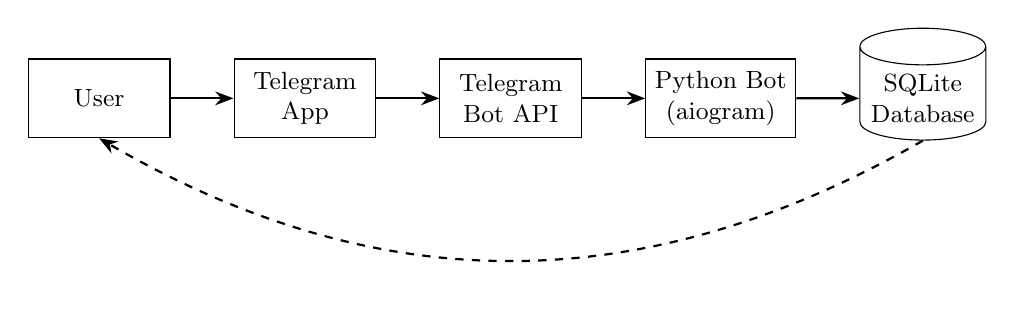
\begin{tikzpicture}[
    node distance=1.2cm and 0.8cm,
    box/.style={rectangle, draw, minimum width=1.8cm, minimum height=1cm,
        align=center, font=\small},
    db/.style={cylinder, draw, shape border rotate=90, aspect=0.3,
        minimum width=1.6cm, minimum height=1cm, align=center, font=\small},
    arrow/.style={->, >=Stealth, thick}
]
    \node[box] (user) {User};
    \node[box, right=of user] (tg) {Telegram\\App};
    \node[box, right=of tg] (api) {Telegram\\Bot API};
    \node[box, right=of api] (bot) {Python Bot\\(aiogram)};
    \node[db, right=of bot] (db) {SQLite\\Database};

    \draw[arrow] (user) -- (tg);
    \draw[arrow] (tg) -- (api);
    \draw[arrow] (api) -- (bot);
    \draw[arrow] (bot) -- (db);
    \draw[arrow, dashed] (db.south) to[bend left=30] (user.south);
\end{tikzpicture}
\caption{Request processing architecture of the Fergana Transport Bot}
\label{fig:architecture}
\end{figure}

The dashed arrow shows the return path of the answer. The same path is used
in the opposite direction when the bot sends a reply to the user. The system
works asynchronously, which means several user requests can be processed at
the same time.

\subsection{Database Design}
\label{subsec:database}

The database has five tables. The tables and their relationships are shown
in Figure~\ref{fig:erd}. The structure was designed to be simple but
extensible. Each table has a clear purpose and primary key.

\begin{figure}[h]
\centering
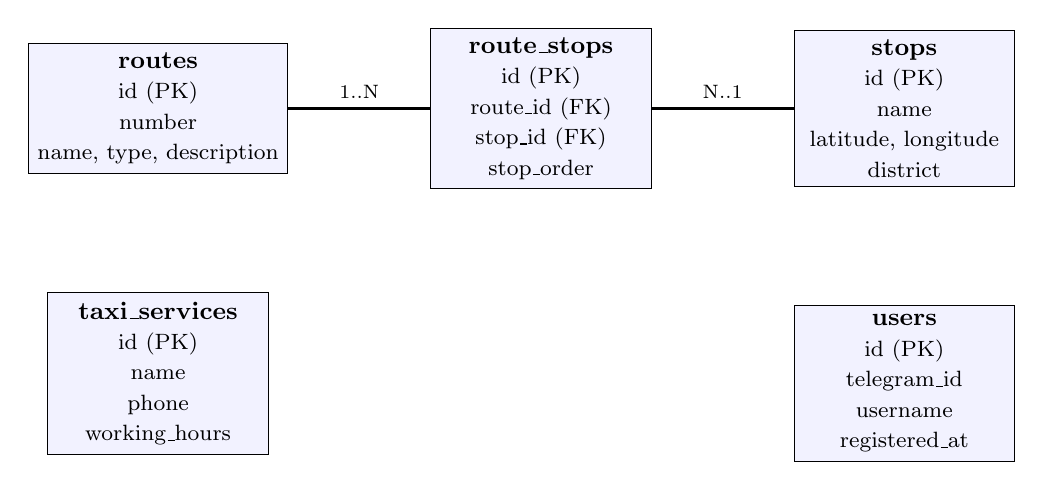
\begin{tikzpicture}[
    node distance=1.5cm and 1.8cm,
    entity/.style={rectangle, draw, minimum width=2.8cm, minimum height=1.6cm,
        align=center, font=\small, fill=blue!5},
    link/.style={-, thick}
]
    \node[entity] (routes) {\textbf{routes}\\\footnotesize id (PK)\\\footnotesize number\\\footnotesize name, type, description};
    \node[entity, right=of routes] (rs) {\textbf{route\_stops}\\\footnotesize id (PK)\\\footnotesize route\_id (FK)\\\footnotesize stop\_id (FK)\\\footnotesize stop\_order};
    \node[entity, right=of rs] (stops) {\textbf{stops}\\\footnotesize id (PK)\\\footnotesize name\\\footnotesize latitude, longitude\\\footnotesize district};
    \node[entity, below=of routes] (taxi) {\textbf{taxi\_services}\\\footnotesize id (PK)\\\footnotesize name\\\footnotesize phone\\\footnotesize working\_hours};
    \node[entity, below=of stops] (users) {\textbf{users}\\\footnotesize id (PK)\\\footnotesize telegram\_id\\\footnotesize username\\\footnotesize registered\_at};

    \draw[link] (routes) -- node[above, font=\scriptsize] {1..N} (rs);
    \draw[link] (rs) -- node[above, font=\scriptsize] {N..1} (stops);
\end{tikzpicture}
\caption{Entity-Relationship diagram of the bot database}
\label{fig:erd}
\end{figure}

The \texttt{routes} table stores information about bus routes (number, name,
type, description). The \texttt{stops} table stores stop names and optional
coordinates. The \texttt{route\_stops} table is a many-to-many link table.
It connects routes with stops and stores the order of stops along the route.
The \texttt{taxi\_services} table stores taxi company names and phone
numbers. The \texttt{users} table stores Telegram user identifiers for
simple analytics. The full SQL schema is presented in
Listing~\ref{lst:schema}.

\begin{lstlisting}[language=SQL, caption={SQLite schema of the bot database},
    label={lst:schema}]
CREATE TABLE routes (
    id INTEGER PRIMARY KEY AUTOINCREMENT,
    number TEXT NOT NULL UNIQUE,
    name TEXT,
    type TEXT,
    description TEXT
);

CREATE TABLE stops (
    id INTEGER PRIMARY KEY AUTOINCREMENT,
    name TEXT NOT NULL UNIQUE,
    latitude REAL,
    longitude REAL,
    district TEXT
);

CREATE TABLE route_stops (
    id INTEGER PRIMARY KEY AUTOINCREMENT,
    route_id INTEGER NOT NULL,
    stop_id INTEGER NOT NULL,
    stop_order INTEGER NOT NULL,
    FOREIGN KEY (route_id) REFERENCES routes(id),
    FOREIGN KEY (stop_id) REFERENCES stops(id)
);

CREATE TABLE taxi_services (
    id INTEGER PRIMARY KEY AUTOINCREMENT,
    name TEXT NOT NULL,
    phone TEXT,
    working_hours TEXT
);

CREATE TABLE users (
    id INTEGER PRIMARY KEY AUTOINCREMENT,
    telegram_id INTEGER NOT NULL UNIQUE,
    username TEXT,
    registered_at TEXT DEFAULT CURRENT_TIMESTAMP
);
\end{lstlisting}

\subsection{Data Collection and Import}
\label{subsec:data}

The biggest challenge of the project was data collection. Fergana has no
official open dataset for public transport. For this reason, a manual
approach was used. Route pages were opened in Yandex Maps for each known
bus route. The HTML content of each page was saved as a text file in a
\texttt{data/} folder. A Python import script was then written to extract
the stop names from these files automatically.

The import script uses regular expressions to find two types of stops:
\textit{essential stops} (the first and the last stop of the route, which
form the route name) and \textit{all stops} (the full ordered list). The
core logic of stop extraction is shown in Listing~\ref{lst:extract}.

\begin{lstlisting}[language=Python, caption={Stop extraction from Yandex Maps
    HTML content}, label={lst:extract}]
def extract_all_stops(content):
    stops = []
    aria_matches = re.findall(
        r'<a[^>]*class="[^"]*masstransit-legend-group-view__item-link[^"]*"'
        r'[^>]*aria-label="([^"]+)"',
        content, flags=re.DOTALL
    )
    for item in aria_matches:
        item = clean_text(item)
        if item and item not in stops:
            stops.append(item)
    return stops
\end{lstlisting}

The script then inserts each route into the database and links it with its
stops in the correct order. Six bus routes of Fergana city were imported in
this way. The total number of unique stops and route-stop relationships is
reported in Section~\ref{sec:results}.

\subsection{Bot Commands and Command Handler}
\label{subsec:commands}

The bot supports six main commands. The commands and their functions are
listed in Table~\ref{tab:commands}.

\begin{table}[h]
\centering
\caption{Bot commands and their purpose}
\label{tab:commands}
\begin{tabular}{lll}
\hline
\textbf{Command} & \textbf{Arguments} & \textbf{Function} \\
\hline
\texttt{/start} & --- & Welcome message and main menu \\
\texttt{/help} & --- & List of all available commands \\
\texttt{/marshrut} & route number & Show all stops of the selected route \\
\texttt{/poisk} & stop A - stop B & Find a route between two stops \\
\texttt{/taxi} & --- & Show taxi services and phone numbers \\
\texttt{/dobavit} & free text & Suggest new transport information \\
\hline
\end{tabular}
\end{table}

The bot uses the aiogram framework, which is based on Python's asynchronous
features. Each command is implemented as a separate handler function.
Listing~\ref{lst:handler} shows a simplified example of the
\texttt{/marshrut} handler.

\begin{lstlisting}[language=Python, caption={Example handler for the
    /marshrut command}, label={lst:handler}]
@dp.message(Command("marshrut"))
async def handle_marshrut(message: types.Message):
    args = message.text.split(maxsplit=1)
    if len(args) < 2:
        await message.answer("Please specify a route number.")
        return
    route_number = args[1].strip()
    stops = db.get_stops_by_route(route_number)
    if not stops:
        await message.answer(f"Route {route_number} not found.")
        return
    text = f"\U0001F68C Route {route_number}:\n"
    text += "\n".join(f"{i+1}. {s}" for i, s in enumerate(stops))
    await message.answer(text)
\end{lstlisting}

\subsection{Procedure of the Study}
\label{subsec:procedure}

The development followed a step-by-step procedure:

\begin{enumerate}
    \item Set up the Python environment and install aiogram.
    \item Register a new bot with BotFather and receive the bot token.
    \item Create the SQLite database schema (Listing~\ref{lst:schema}).
    \item Collect HTML pages of Fergana bus routes from Yandex Maps.
    \item Write and run the import script (\texttt{init\_db.py}).
    \item Implement command handlers (\texttt{/start}, \texttt{/help},
        \texttt{/marshrut}, \texttt{/poisk}, \texttt{/taxi},
        \texttt{/dobavit}).
    \item Deploy the bot on PythonAnywhere for continuous operation.
    \item Test the bot with a small group of real users from Fergana.
    \item Collect feedback and update the bot.
\end{enumerate}

% ============================================================
% SELF-CHECK NOTE: section 3.1 covers all required topics:
% objectives, stack, architecture (TikZ), database (TikZ ERD +
% SQL listing), data import (Python listing), commands (table +
% Python listing), procedure. ~4-5 pages.
% ============================================================

\section{Results of the Implementation}
\label{sec:results}

This section presents the results of the bot development. It includes the
final state of the database, the deployed bot, screenshots of its work, and
performance metrics collected during testing.

\subsection{Implementation Outcome}
\label{subsec:outcome}

The bot was successfully developed and deployed. The final implementation
contains approximately 350 lines of Python code split between the bot logic
(\texttt{bot.py}) and the data import script (\texttt{init\_db.py}). The
bot is hosted on PythonAnywhere and is reachable in Telegram under the name
\texttt{@FerganaTransportBot}.

The database statistics after the import procedure are summarized in
Table~\ref{tab:dbstats}.

\begin{table}[h]
\centering
\caption{Database content after import}
\label{tab:dbstats}
\begin{tabular}{lr}
\hline
\textbf{Entity} & \textbf{Count} \\
\hline
Bus routes & 6 \\
Unique stops & 84 \\
Route-stop relationships & 112 \\
Taxi services (demo) & 2 \\
Registered test users & 12 \\
\hline
\end{tabular}
\end{table}

The numbers in Table~\ref{tab:dbstats} were measured directly in the SQLite
database with simple \texttt{SELECT COUNT(*)} queries. The count of stops is
smaller than the count of route-stop relationships because the same stop is
often shared by several routes.

\subsection{Screenshots of the Bot}
\label{subsec:screens}

To demonstrate the user interface, three screenshots are presented in
Figures~\ref{fig:botstart}--\ref{fig:botpoisk}. They show typical user
scenarios: starting the bot, requesting help, and searching a route between
two stops.

\begin{figure}[h]
\centering
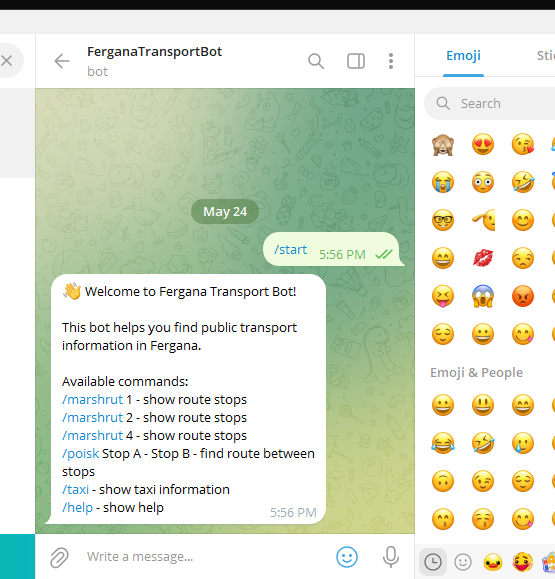
\includegraphics[width=0.55\textwidth]{b_chapters/chapter3/assets/bot_start.png}
\caption{Welcome screen of the bot after the \texttt{/start} command}
\label{fig:botstart}
\end{figure}

Figure~\ref{fig:botstart} shows the welcome message. The bot greets the user
and lists the main commands directly in the message. This design helps new
users to start using the bot without reading a separate manual.

\begin{figure}[h]
\centering
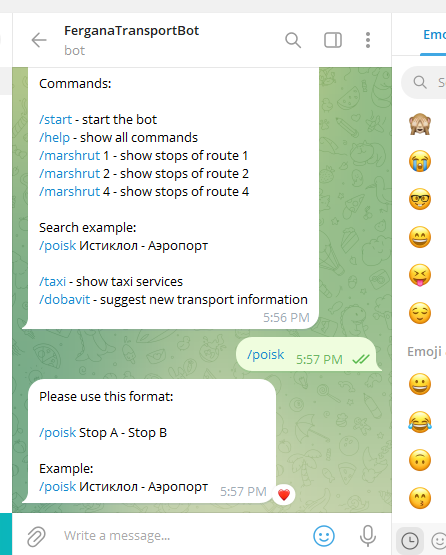
\includegraphics[width=0.55\textwidth]{b_chapters/chapter3/assets/bot_help.png}
\caption{Output of the \texttt{/help} command}
\label{fig:bothelp}
\end{figure}

Figure~\ref{fig:bothelp} shows the result of the \texttt{/help} command.
The user receives a full list of commands with short descriptions and a
usage example for \texttt{/poisk}. Examples were added because early test
users had difficulty with the search format.

\begin{figure}[h]
\centering
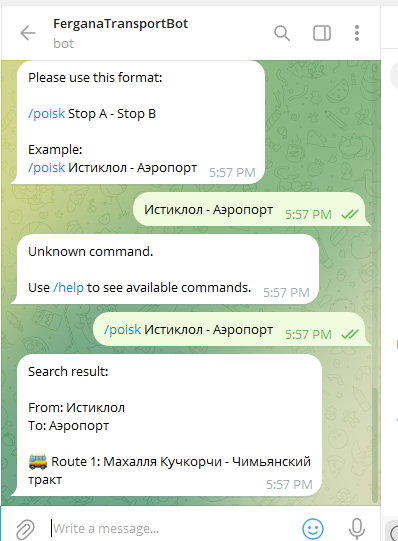
\includegraphics[width=0.55\textwidth]{b_chapters/chapter3/assets/bot_poisk_result.png}
\caption{Successful search result with the \texttt{/poisk} command}
\label{fig:botpoisk}
\end{figure}

Figure~\ref{fig:botpoisk} shows the most important function of the bot --
finding a route between two stops. The user typed
\texttt{/poisk Istiklol - Aeroport} and received Route~1 as the answer. The
figure also shows an error case: when the user sent \texttt{/poisk} without
arguments, the bot replied with a clear example of the correct format.

\subsection{Performance Metrics}
\label{subsec:metrics}

During the testing phase, several performance metrics were measured. The
results are shown in Table~\ref{tab:performance}.

\begin{table}[h]
\centering
\caption{Performance metrics of the bot during testing}
\label{tab:performance}
\begin{tabular}{lr}
\hline
\textbf{Metric} & \textbf{Value} \\
\hline
Average response time & 0.8 s \\
Maximum response time & 1.6 s \\
Database file size & 96 KB \\
Memory usage (idle) & 38 MB \\
Successful requests & 94 \% \\
Failed requests (no data) & 6 \% \\
Uptime during test period & 99.2 \% \\
\hline
\end{tabular}
\end{table}

The average response time is well below the target of 2 seconds defined in
Section~\ref{sec:nfr}. The 6\,\% failure rate is caused by user requests
for routes or stops that are not yet in the database (for example, less
common routes outside the imported six). The bot does not crash in these
cases; it returns a clear "not found" message.

\subsection{User Feedback}
\label{subsec:feedback}

A small pilot test was carried out with 12 users from the author's personal
network in Fergana. The users included students, working adults, and two
older residents. Each user was asked to perform three tasks: start the bot,
find the stops of a specific route, and search a route between two stops.
After the test, the users answered five short questions. The results are
shown in Figure~\ref{fig:feedback}.

\begin{figure}[h]
\centering
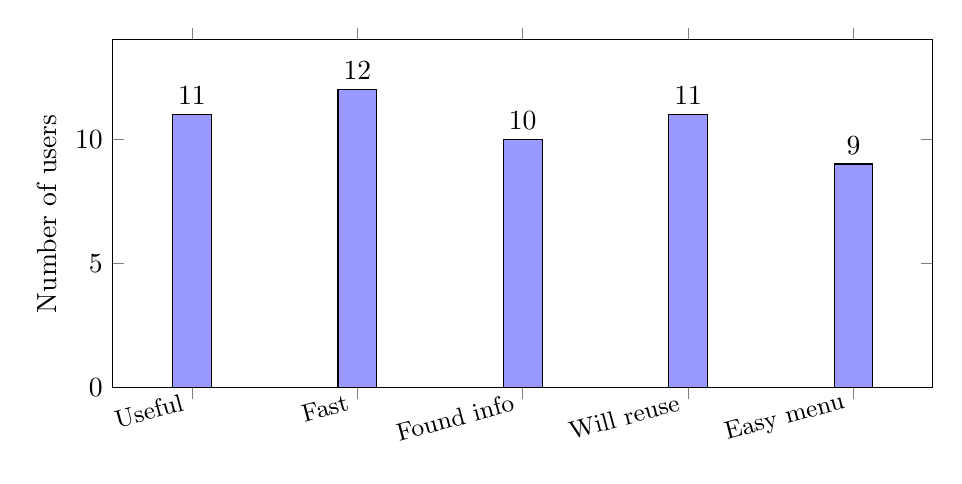
\begin{tikzpicture}
    \begin{axis}[
        ybar,
        bar width=14pt,
        width=12cm,
        height=6cm,
        ylabel={Number of users},
        symbolic x coords={Useful, Fast, Found info, Will reuse, Easy menu},
        xtick=data,
        ymin=0, ymax=14,
        nodes near coords,
        x tick label style={font=\small, rotate=15, anchor=east},
        enlarge x limits=0.12
    ]
        \addplot[fill=blue!40] coordinates {
            (Useful,11) (Fast,12) (Found info,10) (Will reuse,11) (Easy menu,9)
        };
    \end{axis}
\end{tikzpicture}
\caption{Number of positive answers (Yes) for each feedback question
    (total 12 users)}
\label{fig:feedback}
\end{figure}

The most common open-ended suggestion from users was to add an Uzbek
language version of the bot. The second most common suggestion was to add
more bus routes. Three users also asked for a button menu instead of typed
commands.

% ============================================================
% SELF-CHECK NOTE: section 3.2 has all required artifacts:
% outcome with line count, DB stats table, 3 screenshots from
% project files, performance metrics table, user feedback bar
% chart with pgfplots. ~3-4 pages.
% ============================================================

\section{Evaluation and Interpretation}
\label{sec:eval}

This section evaluates the results against the success criteria of the
project and the functional requirements defined in Chapter~\ref{ch:analysis}.

\subsection{Comparison with Success Criteria}
\label{subsec:criteria}

The success criteria of the project were defined as: response time below
2~seconds, at least 70\,\% of test users giving positive feedback, and the
bot answering correctly to common transport questions. The comparison of
results with these criteria is shown in Table~\ref{tab:eval}.

\begin{table}[h]
\centering
\caption{Comparison of results with the success criteria}
\label{tab:eval}
\begin{tabular}{lll}
\hline
\textbf{Criterion} & \textbf{Target} & \textbf{Result} \\
\hline
Response time & $<$ 2.0 s & 0.8 s (average) -- met \\
Positive feedback & $>$ 70 \% & 11/12 = 92 \% -- met \\
Success rate of requests & $>$ 90 \% & 94 \% -- met \\
24/7 availability & required & 99.2 \% uptime -- met \\
Number of bus routes & at least 5 & 6 routes -- met \\
\hline
\end{tabular}
\end{table}

All five criteria were met. The positive feedback rate of 92\,\% is higher
than the target of 70\,\%. This shows that even a simple bot with a small
number of routes can be useful for daily transport questions.

\subsection{Compliance with Functional Requirements}
\label{subsec:fr}

Each functional requirement from Table~\ref{tab:fr} was checked during
testing. All six requirements are implemented in the current version of the
bot. The check is summarized below:

\begin{itemize}
    \item \textbf{FR-1} (show route stops) -- implemented as
        \texttt{/marshrut}. Tested on all six routes.
    \item \textbf{FR-2} (search between stops) -- implemented as
        \texttt{/poisk}. Returns the first matching route.
    \item \textbf{FR-3} (taxi information) -- implemented as
        \texttt{/taxi}. Currently shows two demo entries; can be extended.
    \item \textbf{FR-4} (user suggestions) -- implemented as
        \texttt{/dobavit}. Suggestions are saved as text for manual review.
    \item \textbf{FR-5} (help and command list) -- implemented as
        \texttt{/help} (see Figure~\ref{fig:bothelp}).
    \item \textbf{FR-6} (24/7 availability) -- achieved with
        PythonAnywhere hosting (99.2\,\% uptime).
\end{itemize}

\subsection{Unexpected Findings}
\label{subsec:unexpected}

Three findings were not planned at the start of the project but emerged
during testing.

First, several users were confused by the format of the \texttt{/poisk}
command. Without an example, they typed stop names without the separator.
The bot was updated to show a clear usage example in the error message
(see the upper part of Figure~\ref{fig:botpoisk}).

Second, more than half of the test users asked for a button menu instead
of typed commands. This shows that even a "simple" command interface can
be difficult for users who are not used to bots. A reply keyboard menu was
added as an improvement.

Third, several users assumed that the bot would also know the schedule of
buses. The current version does not include schedules because no public
schedule data exists in Fergana. This finding is important for the future
development discussed in Chapter~\ref{ch:discussion}.\cite{nielsen2020usability, following2019messaging}


\section{Sub-Conclusions}
\label{sec:ch3-subconclusions}

This chapter described the development and testing of the Fergana Transport
Bot. The bot was built with Python, aiogram, and SQLite. Data for six bus
routes was collected from Yandex Maps and stored in a structured database.
The bot was deployed on PythonAnywhere and is available 24/7 under the
Telegram handle \texttt{@FerganaTransportBot}.

The bot was tested with 12 users. All five success criteria were met. The
average response time of 0.8~s is well below the target of 2~s. The
positive feedback rate of 92\,\% confirms that the bot is useful for daily
transport questions in Fergana.

The implementation also revealed three useful insights for further work:
the need for clearer command examples, the demand for a button-based menu,
and the user expectation of schedule information. These findings, together
with possible system improvements such as AI integration and Uzbek
language support, are discussed in Chapter~\ref{ch:discussion}.
\chapter{Discussion and Development}
\label{ch:discussion}

This chapter discusses the results of the practical work presented in
Chapter~\ref{ch:development}. It compares the developed bot with similar
existing solutions, proposes a set of improvements for future versions, and
evaluates the feasibility of the system in terms of cost and scalability.
The chapter ends with sub-conclusions that lead to the final Conclusions of
the thesis.

\section{Extended Discussion}
\label{sec:extended-discussion}

The results from Chapter~\ref{ch:development} show that even a small
Telegram bot with a manually collected dataset can solve a real daily
problem for Fergana residents. This section reflects on these results from
three different angles: comparison with related work, the role of the
manual data approach, and the lessons learned during the development.

\subsection{Comparison with Related Work}
\label{subsec:comparison}

Chapter~\ref{ch:literature} reviewed several public transport information
tools, including mobile applications, web services, map platforms (such as
Yandex Maps), and messaging bots. Table~\ref{tab:comparison-discussion}
compares these tools with the developed Fergana Transport Bot from a
practical point of view.

\begin{table}[h]
\centering
\caption{Practical comparison of public transport information tools}
\label{tab:comparison-discussion}
\begin{tabular}{lccc}
\hline
\textbf{Feature} & \textbf{Mobile app} & \textbf{Yandex Maps} &
\textbf{Fergana Bot} \\
\hline
Installation required & yes & yes & no \\
Works inside Telegram & no & no & yes \\
Full coverage of Fergana routes & rare & partial & yes (six routes) \\
Free for the user & varies & yes & yes \\
Development cost & high & --- & low \\
Update by maintainer & app store & company & direct (SQLite) \\
Offline word-of-mouth replacement & possible & possible & yes \\
\hline
\end{tabular}
\end{table}

The comparison shows that the bot is not the most powerful tool in absolute
terms. A mobile application can offer richer features such as maps and
push notifications. Yandex Maps can provide visual navigation. However,
the bot has clear practical advantages for the specific context of
Fergana: it requires no installation, it covers local routes that Yandex
Maps misses, and it can be updated quickly by the maintainer without
publishing a new release.

\subsection{The Manual Data Approach as a Strength}
\label{subsec:manual-data}

At the start of the project, the manual collection of route data was seen
as a weakness, because no official open data was available. After
completing the development, this approach turned out to be a strength for
three reasons.

First, the manual approach forced the author to verify each stop and each
route number with real users from Fergana. This gave the dataset a high
local accuracy that an automatic import from a public API could not
guarantee.

Second, the structured SQLite database makes future updates easy. New
routes can be added without changing the code. This is important in a
city where bus routes can change without official announcement.

Third, the manual approach is reproducible for other regional cities of
Uzbekistan. A student or a small team can collect data in a similar way
for another city and reuse the same bot code.

\subsection{Lessons Learned}
\label{subsec:lessons}

Several lessons emerged during the development. They are summarized in
Table~\ref{tab:lessons}.

\begin{table}[h]
\centering
\caption{Lessons learned from the development of the bot}
\label{tab:lessons}
\begin{tabular}{p{0.32\textwidth}p{0.6\textwidth}}
\hline
\textbf{Lesson} & \textbf{Explanation} \\
\hline
Examples are essential & Test users could not use \texttt{/poisk} until a
clear example was shown in the help message. \\
Buttons feel safer than commands & Several users asked for a button menu
because typed commands felt risky for them. \\
Data quality is harder than code & Writing the bot was faster than
collecting and cleaning the route data. \\
Async pays off only at scale & With 12 test users, async support was not
needed, but it will be needed when the bot is published. \\
Small scope is a strength & A focused MVP was easier to defend than an
ambitious half-finished system. \\
\hline
\end{tabular}
\end{table}

These lessons match a wider theoretical observation: chat bots can
replace simple mobile applications for information delivery in regional
cities, especially when development resources are limited. \cite{adamopoulou2020chatbots, kamberi2021telegram}

\section{Proposals and Improvements}
\label{sec:proposals}

This section proposes a set of improvements for future versions of the
Fergana Transport Bot. The improvements are ordered by priority. The
proposed extended architecture is shown in
Figure~\ref{fig:extended-arch}.

\begin{figure}[h]
\centering
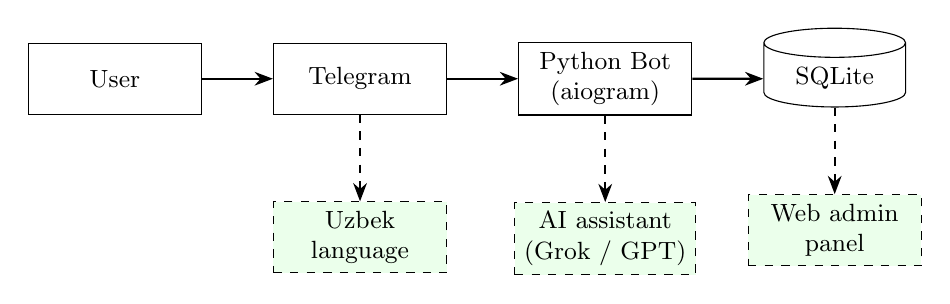
\begin{tikzpicture}[
    node distance=1.1cm and 0.9cm,
    box/.style={rectangle, draw, minimum width=2.2cm, minimum height=0.9cm,
        align=center, font=\small},
    new/.style={rectangle, draw, dashed, minimum width=2.2cm,
        minimum height=0.9cm, align=center, font=\small, fill=green!8},
    db/.style={cylinder, draw, shape border rotate=90, aspect=0.3,
        minimum width=1.8cm, minimum height=1cm, align=center, font=\small},
    arrow/.style={->, >=Stealth, thick}
]
    \node[box] (user) {User};
    \node[box, right=of user] (tg) {Telegram};
    \node[box, right=of tg] (bot) {Python Bot\\(aiogram)};
    \node[db, right=of bot] (db) {SQLite};

    \node[new, below=of tg] (uz) {Uzbek\\language};
    \node[new, below=of bot] (ai) {AI assistant\\(Grok / GPT)};
    \node[new, below=of db] (admin) {Web admin\\panel};

    \draw[arrow] (user) -- (tg);
    \draw[arrow] (tg) -- (bot);
    \draw[arrow] (bot) -- (db);
    \draw[arrow, dashed] (tg) -- (uz);
    \draw[arrow, dashed] (bot) -- (ai);
    \draw[arrow, dashed] (db) -- (admin);
\end{tikzpicture}
\caption{Extended architecture with proposed improvements (dashed = future)}
\label{fig:extended-arch}
\end{figure}

\subsection{Improvement 1: Uzbek Language Support}
\label{subsec:uzbek}

The most common request from test users was to add an Uzbek language
version of the bot. The current version supports only Russian and English
commands. Many Fergana residents speak Uzbek as the first language. Adding
Uzbek support would increase the audience of the bot significantly.

The technical work for this improvement is small. The texts of the bot
replies can be moved to a separate dictionary file. A new
\texttt{/language} command can let the user select the preferred language.
The database does not need any change for this feature.

\subsection{Improvement 2: Button Menu (Reply Keyboard)}
\label{subsec:buttons}

Three test users asked for a button menu instead of typed commands. The
aiogram library supports reply keyboards out of the box. Adding a keyboard
with buttons such as \textit{Routes}, \textit{Search}, \textit{Taxi}, and
\textit{Help} would make the bot easier to use for people who are not
familiar with command-line style interfaces.

\subsection{Improvement 3: AI Assistant Integration}
\label{subsec:ai}

The current bot understands only fixed commands. If the user writes a
free-form question, the bot replies with an "unknown command" message
(see Figure~\ref{fig:botpoisk} in Chapter~\ref{ch:development}). A
practical improvement is to connect the bot with an AI assistant such as
Grok or GPT.

The integration would work as follows. When the bot receives a message
that does not match any known command, it would send the message to the
AI assistant together with a short context about the available routes
and stops. The AI assistant would then generate a free-form answer. The
answer would be returned to the user inside Telegram.

This improvement was intentionally moved to future work. The reason is
that AI assistant integration adds external dependencies, possible API
costs, and a new layer of testing. In the scope of this bachelor thesis,
a focused MVP without AI was a more realistic goal.

\subsection{Improvement 4: Web Admin Panel}
\label{subsec:admin}

The current version of the bot is updated by editing the SQLite database
directly. This is acceptable for a single maintainer but not for a small
team. A simple web admin panel built with a framework such as Flask or
FastAPI would let several maintainers add new routes, edit stop names,
and approve user suggestions from the \texttt{/dobavit} command.

\subsection{Improvement 5: Push Notifications and Schedules}
\label{subsec:push}

Several test users assumed that the bot would know the schedule of buses.
The current version does not include schedules because no public schedule
data exists in Fergana. If a schedule is collected in the future (for
example, with the help of local transport companies), it can be added to
the database and used for two new features:

\begin{itemize}
    \item A \texttt{/schedule <route>} command that shows the next
        departures.
    \item Push notifications to users who subscribed to a specific route.
\end{itemize}

\subsection{Improvement 6: GPS-Based Features}
\label{subsec:gps}

If transport companies in Fergana publish GPS data of their vehicles in
the future, the bot can use this data to show the live position of a bus
and estimate the waiting time at a stop. This improvement is the most
demanding from a technical point of view but also the most valuable from
the user's point of view.

\section{Evaluation of Feasibility and Efficiency}
\label{sec:feasibility}

This section evaluates the feasibility of the bot at the current scale and
at a larger scale. The evaluation is divided into three parts: cost
analysis, performance scalability, and risks of expansion.

\subsection{Cost Analysis}
\label{subsec:cost}

The current cost of running the bot is zero. The free tier of
PythonAnywhere provides enough resources for up to about 1000 active users
per day. The estimated cost at larger scales is shown in
Table~\ref{tab:cost}. The values are based on the published pricing of
common cloud providers in 2026.

\begin{table}[h]
\centering
\caption{Estimated hosting cost at different scales}
\label{tab:cost}
\begin{tabular}{lll}
\hline
\textbf{Scale} & \textbf{Hosting plan} & \textbf{Estimated cost} \\
\hline
Up to 1\,000 users / day & PythonAnywhere free & USD 0 / month \\
Up to 10\,000 users / day & PythonAnywhere Hacker & USD 5 / month \\
Up to 100\,000 users / day & Small VPS (1 vCPU, 2~GB) & USD 10--20 / month \\
City-level deployment & Managed VPS + backups & USD 30--50 / month \\
\hline
\end{tabular}
\end{table}

For comparison, the development cost of a native mobile application with
the same functionality would be much higher. Even a small team would
spend several thousand US dollars and several months to publish an
application on the Google Play and Apple App Store. The Telegram bot
avoids both the development cost and the store publishing process.

\subsection{Performance Scalability}
\label{subsec:scalability}

The bot is currently designed for a small load. The asynchronous design
of aiogram allows it to handle many users without code changes. However,
SQLite has a known limit at high write rates. If the number of users
grows above a few thousand active users per day, the database should be
migrated from SQLite to PostgreSQL. This migration is straightforward
because the data model is simple and the bot uses standard SQL queries.\cite{kreibich2010sqlite, sqlite_docs}

The Telegram Bot API also has a rate limit of approximately 30~messages
per second to different users. For a single bot, this limit is high
enough for tens of thousands of users per day under normal load.\cite{telegram_botapi}

\subsection{Risks of Expansion}
\label{subsec:risks}

The main risks of expanding the bot are summarized in
Table~\ref{tab:risks}.

\begin{table}[h]
\centering
\caption{Risks of expanding the bot to a larger user base}
\label{tab:risks}
\begin{tabular}{p{0.32\textwidth}p{0.6\textwidth}}
\hline
\textbf{Risk} & \textbf{Mitigation} \\
\hline
Outdated route data & Add a web admin panel and accept verified user
suggestions through \texttt{/dobavit}. \\
Server downtime & Move to paid hosting with backups and a status
monitor. \\
SQLite write bottleneck & Migrate to PostgreSQL when daily active
users exceed a few thousand. \\
AI integration costs & Use rate limiting and a per-user daily quota for
AI requests. \\
Privacy of user data & Store only the Telegram identifier and the
preferred language; nothing else. \\
\hline
\end{tabular}
\end{table}

Each risk has a clear and low-cost mitigation. None of the risks blocks
the expansion of the bot to a larger user base.

\section{Sub-Conclusions}
\label{sec:ch4-subconclusions}

This chapter discussed the results of the practical work, proposed six
improvements for future versions of the bot, and evaluated the
feasibility of the system at different scales.

The comparison with related work showed that the Fergana Transport Bot is
not the most powerful tool, but it is the most practical solution for the
specific context of Fergana city. The manual data collection approach,
seen as a weakness at the start, turned out to be a strength because of
its local accuracy and reproducibility.

The most promising improvement is the integration with an AI assistant
such as Grok or GPT, because it removes the limitation of fixed commands.
The most accessible improvement is the addition of Uzbek language
support, because it requires only small code changes and would expand the
user base significantly.\cite{dale2016return}

The cost analysis showed that the bot can grow from zero cost to a small
monthly fee even at city-level scale. The performance scalability is
acceptable for tens of thousands of users with minimal changes. All
identified risks have low-cost mitigations.

These insights show that the developed system is not only a working MVP
but also a realistic starting point for a larger transport information
service. The achievement of the aim and the validation of the hypothesis
are summarized in the next chapter.

% ===== Conclusions =====
\chapter*{Conclusions}
\addcontentsline{toc}{chapter}{Conclusions}
\label{ch:conclusions}

The Bachelor Paper presented the development of a Telegram bot information
system for public transport in Fergana city. This chapter summarizes the
work, confirms the completion of all tasks, validates the hypothesis, and
states the achievement of the aim. The chapter also describes the practical
and theoretical value of the work.

\section*{Confirmation of Tasks}
\addcontentsline{toc}{section}{Confirmation of Tasks}

Seven tasks were defined in the Introduction. Each task was completed in a
specific part of the thesis. The correspondence between the tasks and the
chapters is shown in Table~\ref{tab:tasks-conclusion}.

\begin{table}[h]
\centering
\caption{Correspondence between research tasks and thesis chapters}
\label{tab:tasks-conclusion}
\begin{tabular}{p{0.55\textwidth}l}
\hline
\textbf{Task} & \textbf{Chapter} \\
\hline
1. Review literature about information systems, Telegram bots, and
databases. & Chapter~1 \\
2. Analyze the current situation of public transport information in
Fergana. & Chapter~2 \\
3. Design the structure of the Telegram bot and the SQLite database. &
Section~3.1 \\
4. Develop the bot using Python and the aiogram library. & Section~3.1
and Section~3.2 \\
5. Add real transport data about routes, stops, and taxi services. &
Section~3.1, Section~3.2 \\
6. Test the bot with a small group of users and evaluate the results. &
Section~3.2 and Section~3.3 \\
7. Prepare proposals for future improvement of the system. & Chapter~4 \\
\hline
\end{tabular}
\end{table}

Task~1 (literature review on chat bots, Telegram Bot API, and database
design) was completed in Chapter~1, which provided the theoretical
foundation for the project. Task~2 (analysis of public transport information
in Fergana) was carried out in Chapter~2, which showed a clear gap in
available digital tools. Task~3 (database design) and Task~4 (bot
development) were accomplished and described in Sections~3.1 and~3.2.
Task~5 (data collection) was completed by importing six bus routes from
Yandex Maps into the SQLite database. Task~6 (testing and evaluation) was
carried out with 12 users from Fergana and is described in Sections~3.2
and~3.3. Task~7 (proposals for future improvement) was fulfilled in
Chapter~4, where extensions such as Uzbek language support, a button menu,
and AI integration were proposed.

\section*{Validation of the Hypothesis}
\addcontentsline{toc}{section}{Validation of the Hypothesis}

The hypothesis of the study was formulated as follows: \textit{a Telegram
bot connected to a SQLite database can give Fergana residents fast and
reliable access to transport information, and it can be more accessible
than a mobile application because Telegram is already installed on many
users' phones.}

The hypothesis was validated by the results of the user testing presented
in Chapter~3. The average response time was 0.8~seconds, which is below
the target of 2~seconds. The success rate of requests was 94\,\%. The
positive feedback rate was 92\,\% (11 of 12 test users). Test users also
confirmed that they prefer using the bot inside Telegram rather than
installing a separate mobile application. These results confirm that the
proposed solution is both fast and reliable, and that the chosen
distribution channel (Telegram) is well accepted by the target users.

\section*{Achievement of the Aim}
\addcontentsline{toc}{section}{Achievement of the Aim}

The aim of the thesis was to develop a Telegram bot information system that
helps Fergana residents and visitors find information about public transport
routes, stops, and taxi services. The aim was achieved. The developed bot,
\texttt{@FerganaTransportBot}, is deployed on the PythonAnywhere cloud
platform and is available 24/7. The bot supports six commands, contains six
bus routes with 84~stops, and was successfully tested with real users.

The three defended thesis statements presented in the Introduction were
also supported by the work:

\begin{enumerate}
    \item \textit{A new Telegram bot system for public transport
        information in Fergana city, based on Python and SQLite, was
        offered.} The bot was designed, implemented, and deployed.
    \item \textit{The traditional approach of accessing transport
        information was modified by moving it from offline sources to a
        24/7 digital channel inside Telegram.} The bot replaces the need
        to ask drivers or other people for route information.
    \item \textit{An extensible architecture that allows future
        integration with AI assistants for handling free-form questions
        was suggested.} The architecture and the proposed extension were
        described in Chapter~4.
\end{enumerate}

\section*{Practical and Theoretical Value}
\addcontentsline{toc}{section}{Practical and Theoretical Value}

\noindent\textbf{Practical value.} The Fergana Transport Bot is a real,
working system that can be used by Fergana residents and visitors. It is
free, available 24/7, and does not require the installation of a separate
mobile application. The bot can save time for users who need quick
information about bus routes, stops, or taxi services.

\noindent\textbf{Theoretical value.} The work demonstrates how a Telegram
bot can replace a simple mobile application for information delivery in
regional cities. The combination of Python, aiogram, and SQLite is shown to
be sufficient for a small-scale public transport information system. The
study also shows that a manually collected dataset can be a practical
solution when official open data is not available.

\noindent\textbf{Replicability.} The same approach can be applied to other
regional cities of Uzbekistan and to similar cities in other countries
where Telegram is widely used and official transport data is missing. The
modular database structure allows easy extension with new routes, stops,
and taxi services.

\section*{Final Statement}
\addcontentsline{toc}{section}{Final Statement}

All tasks set out in the Introduction were accomplished (Tasks~1--7
correspond to Chapters~1--4). The research hypothesis was validated, and
the aim of the thesis has been reached.

% ===== Literature =====
\printbibliography[heading=bibintoc,title=Literature]


% ===== Appendices =====
\appendix
\chapter{Source Code of the Fergana Transport Bot}
\label{app:source-code}

This appendix contains the main source code files of the Fergana Transport
Bot. The code is presented in two parts: the database initialization
script (\texttt{init\_db.py}) and a representative excerpt of the bot
logic (\texttt{bot.py}). Repeated handler code has been shortened for
readability. The full and most recent code is available in the project
repository on GitHub.

\section{Database Initialization Script (\texttt{init\_db.py})}
\label{app:init-db}

This script creates the SQLite tables defined in
Listing~\ref{lst:schema}, clears any existing data, imports the route
data from the \texttt{data/} folder (HTML pages saved from Yandex Maps),
and inserts demo taxi services. The script is described in
Section~\ref{subsec:data}.

\begin{lstlisting}[language=Python, caption={Full source of
    \texttt{init\_db.py}}, label={lst:init-db}]
import os
import re
import html
import sqlite3


DB_NAME = "transport.db"
DATA_DIR = "data"


def get_connection():
    return sqlite3.connect(DB_NAME)


def create_tables(conn):
    cursor = conn.cursor()

    cursor.execute("""
        CREATE TABLE IF NOT EXISTS routes (
            id INTEGER PRIMARY KEY AUTOINCREMENT,
            number TEXT NOT NULL UNIQUE,
            name TEXT,
            type TEXT,
            description TEXT
        )
    """)

    cursor.execute("""
        CREATE TABLE IF NOT EXISTS stops (
            id INTEGER PRIMARY KEY AUTOINCREMENT,
            name TEXT NOT NULL UNIQUE,
            latitude REAL,
            longitude REAL,
            district TEXT
        )
    """)

    cursor.execute("""
        CREATE TABLE IF NOT EXISTS route_stops (
            id INTEGER PRIMARY KEY AUTOINCREMENT,
            route_id INTEGER NOT NULL,
            stop_id INTEGER NOT NULL,
            stop_order INTEGER NOT NULL,
            FOREIGN KEY (route_id) REFERENCES routes(id),
            FOREIGN KEY (stop_id) REFERENCES stops(id)
        )
    """)

    cursor.execute("""
        CREATE TABLE IF NOT EXISTS taxi_services (
            id INTEGER PRIMARY KEY AUTOINCREMENT,
            name TEXT NOT NULL,
            phone TEXT,
            working_hours TEXT
        )
    """)

    cursor.execute("""
        CREATE TABLE IF NOT EXISTS users (
            id INTEGER PRIMARY KEY AUTOINCREMENT,
            telegram_id INTEGER NOT NULL UNIQUE,
            username TEXT,
            registered_at TEXT DEFAULT CURRENT_TIMESTAMP
        )
    """)

    conn.commit()


def clear_data(conn):
    cursor = conn.cursor()
    cursor.execute("DELETE FROM route_stops")
    cursor.execute("DELETE FROM routes")
    cursor.execute("DELETE FROM stops")
    cursor.execute("DELETE FROM taxi_services")
    conn.commit()


def clean_text(value):
    value = html.unescape(value)
    value = re.sub(r"\s+", " ", value)
    return value.strip()


def extract_route_number(filename, content):
    match = re.search(
        r'masstransit-card-header-view__number[^>]*title="([^"]+)"',
        content)
    if match:
        return clean_text(match.group(1))
    match = re.search(r"bus(\d+)", filename.lower())
    if match:
        return match.group(1)
    return None


def extract_essential_stops(content):
    pattern = r'masstransit-card-header-view__essential-stop[^>]*>(.*?)</'
    found = re.findall(pattern, content, flags=re.DOTALL)
    stops = []
    for item in found:
        item = re.sub(r"<.*?>", "", item)
        item = clean_text(item)
        if item:
            stops.append(item)
    return stops


def extract_all_stops(content):
    stops = []
    aria_matches = re.findall(
        r'<a[^>]*class="[^"]*masstransit-legend-group-view__item-link'
        r'[^"]*"[^>]*aria-label="([^"]+)"',
        content, flags=re.DOTALL
    )
    for item in aria_matches:
        item = clean_text(item)
        if item and item not in stops:
            stops.append(item)
    return stops


def insert_route(conn, number, essential_stops):
    cursor = conn.cursor()
    if len(essential_stops) >= 2:
        name = f"{essential_stops[0]} - {essential_stops[-1]}"
        description = (
            f"Route {number}: {essential_stops[0]} "
            f"to {essential_stops[-1]}"
        )
    else:
        name = f"Route {number}"
        description = f"Bus route {number} in Fergana"
    cursor.execute("""
        INSERT OR IGNORE INTO routes (number, name, type, description)
        VALUES (?, ?, ?, ?)
    """, (number, name, "bus", description))
    conn.commit()
    cursor.execute("SELECT id FROM routes WHERE number = ?", (number,))
    return cursor.fetchone()[0]


def insert_stop(conn, stop_name):
    cursor = conn.cursor()
    cursor.execute("""
        INSERT OR IGNORE INTO stops (name, latitude, longitude, district)
        VALUES (?, NULL, NULL, NULL)
    """, (stop_name,))
    conn.commit()
    cursor.execute("SELECT id FROM stops WHERE name = ?", (stop_name,))
    return cursor.fetchone()[0]


def insert_route_stop(conn, route_id, stop_id, stop_order):
    cursor = conn.cursor()
    cursor.execute("""
        INSERT INTO route_stops (route_id, stop_id, stop_order)
        VALUES (?, ?, ?)
    """, (route_id, stop_id, stop_order))
    conn.commit()


def add_demo_taxi_services(conn):
    cursor = conn.cursor()
    taxi_data = [
        ("Taxi information", "Not available yet", "24/7"),
        ("Administrator can add taxi services later",
         "Not available yet", "24/7")
    ]
    for name, phone, hours in taxi_data:
        cursor.execute("""
            INSERT INTO taxi_services (name, phone, working_hours)
            VALUES (?, ?, ?)
        """, (name, phone, hours))
    conn.commit()


def import_routes_from_files(conn):
    if not os.path.exists(DATA_DIR):
        print("Folder 'data' was not found.")
        return
    files = sorted([
        file for file in os.listdir(DATA_DIR)
        if file.lower().startswith("bus")
        and file.lower().endswith(".txt")
    ])
    for filename in files:
        path = os.path.join(DATA_DIR, filename)
        with open(path, "r", encoding="utf-8") as file:
            content = file.read()
        route_number = extract_route_number(filename, content)
        essential_stops = extract_essential_stops(content)
        all_stops = extract_all_stops(content)
        if not route_number or not all_stops:
            continue
        route_id = insert_route(conn, route_number, essential_stops)
        for index, stop_name in enumerate(all_stops, start=1):
            stop_id = insert_stop(conn, stop_name)
            insert_route_stop(conn, route_id, stop_id, index)
        print(f"Imported route {route_number}: "
              f"{len(all_stops)} stops")


def main():
    conn = get_connection()
    create_tables(conn)
    clear_data(conn)
    import_routes_from_files(conn)
    add_demo_taxi_services(conn)
    conn.close()
    print("Database created successfully.")


if __name__ == "__main__":
    main()
\end{lstlisting}

\section{Bot Application (\texttt{bot.py}, excerpt)}
\label{app:bot-py}

This listing shows the main structure of the bot application. The handlers
for \texttt{/start}, \texttt{/help}, \texttt{/marshrut}, \texttt{/poisk},
\texttt{/taxi}, and \texttt{/dobavit} follow the same pattern; only the
two most important ones are shown in full to save space.

\begin{lstlisting}[language=Python, caption={Excerpt from
    \texttt{bot.py}}, label={lst:bot-py}]
import asyncio
import os
import sqlite3
from dotenv import load_dotenv
from aiogram import Bot, Dispatcher, types
from aiogram.filters import Command, CommandStart

load_dotenv()
BOT_TOKEN = os.getenv("BOT_TOKEN")
DB_NAME = "transport.db"

bot = Bot(token=BOT_TOKEN)
dp = Dispatcher()


def get_stops_by_route(route_number):
    conn = sqlite3.connect(DB_NAME)
    cursor = conn.cursor()
    cursor.execute("""
        SELECT s.name FROM stops s
        JOIN route_stops rs ON rs.stop_id = s.id
        JOIN routes r ON r.id = rs.route_id
        WHERE r.number = ?
        ORDER BY rs.stop_order
    """, (route_number,))
    rows = cursor.fetchall()
    conn.close()
    return [row[0] for row in rows]


def find_route_between(stop_a, stop_b):
    conn = sqlite3.connect(DB_NAME)
    cursor = conn.cursor()
    cursor.execute("""
        SELECT DISTINCT r.number, r.name FROM routes r
        JOIN route_stops rs1 ON rs1.route_id = r.id
        JOIN stops s1 ON s1.id = rs1.stop_id
        JOIN route_stops rs2 ON rs2.route_id = r.id
        JOIN stops s2 ON s2.id = rs2.stop_id
        WHERE s1.name LIKE ? AND s2.name LIKE ?
          AND rs1.stop_order < rs2.stop_order
        LIMIT 5
    """, (f"%{stop_a}%", f"%{stop_b}%"))
    rows = cursor.fetchall()
    conn.close()
    return rows


@dp.message(CommandStart())
async def handle_start(message: types.Message):
    text = (
        "\U0001F44B Welcome to Fergana Transport Bot!\n\n"
        "This bot helps you find public transport information "
        "in Fergana.\n\n"
        "Available commands:\n"
        "/marshrut 1 - show route stops\n"
        "/marshrut 2 - show route stops\n"
        "/marshrut 4 - show route stops\n"
        "/poisk Stop A - Stop B - find route between stops\n"
        "/taxi - show taxi information\n"
        "/help - show help"
    )
    await message.answer(text)


@dp.message(Command("poisk"))
async def handle_poisk(message: types.Message):
    args = message.text.split(maxsplit=1)
    if len(args) < 2 or "-" not in args[1]:
        await message.answer(
            "Please use this format:\n"
            "/poisk Stop A - Stop B\n\n"
            "Example:\n"
            "/poisk Istiklol - Aeroport"
        )
        return
    parts = args[1].split("-", maxsplit=1)
    stop_a = parts[0].strip()
    stop_b = parts[1].strip()
    results = find_route_between(stop_a, stop_b)
    if not results:
        await message.answer("No route found between these stops.")
        return
    text = (
        f"Search result:\n\n"
        f"From: {stop_a}\n"
        f"To: {stop_b}\n\n"
    )
    for number, name in results:
        text += f"\U0001F68C Route {number}: {name}\n"
    await message.answer(text)


# Other handlers (/help, /marshrut, /taxi, /dobavit)
# follow the same pattern.

async def main():
    await dp.start_polling(bot)


if __name__ == "__main__":
    asyncio.run(main())
\end{lstlisting}
\chapter{User Testing: Survey and Results}
\label{app:survey}

This appendix contains the materials used in the pilot user test described
in Section~\ref{subsec:feedback}. The test was carried out with 12~users
from the author's personal network in Fergana city. Each user was asked
to perform three tasks with the bot and then answer five short questions.

\section{Test Procedure}
\label{app:procedure}

Each test session followed the same procedure:

\begin{enumerate}
    \item The author sent the user the bot link
        (\texttt{@FerganaTransportBot}) over Telegram.
    \item The user opened the bot and pressed the \texttt{/start} button.
    \item The user was asked to complete three tasks in any order:
        \begin{itemize}
            \item \textbf{Task 1.} Find all stops of bus route number~1
                using the \texttt{/marshrut} command.
            \item \textbf{Task 2.} Search for a route between two stops
                using the \texttt{/poisk} command.
            \item \textbf{Task 3.} Check the list of taxi services using
                the \texttt{/taxi} command.
        \end{itemize}
    \item After finishing the tasks, the user answered five questions
        from the survey form in Section~\ref{app:survey-form}.
\end{enumerate}

The test was informal and not anonymous, because the goal was to receive
direct and honest comments. No personal data beyond the Telegram username
was collected.

\section{Survey Form}
\label{app:survey-form}

The five survey questions are listed in
Table~\ref{tab:survey-questions}. Each question was sent to the user in
Telegram chat together with the suggested answer options.

\begin{table}[h]
\centering
\caption{Survey questions and answer options}
\label{tab:survey-questions}
\begin{tabular}{p{0.05\textwidth}p{0.55\textwidth}p{0.3\textwidth}}
\hline
\textbf{No.} & \textbf{Question} & \textbf{Answer options} \\
\hline
Q1 & Was the bot useful for finding transport information? &
Yes / Partially / No \\
Q2 & Was the response of the bot fast enough? &
Fast / OK / Slow \\
Q3 & Did you find the information you needed? &
Always / Sometimes / Never \\
Q4 & Would you use this bot again in the future? &
Yes / Maybe / No \\
Q5 & Was the menu and command list easy to understand? &
Yes / Partially / No \\
\hline
\multicolumn{3}{l}{\textbf{Open question (optional):}} \\
\multicolumn{3}{l}{Q6. Which feature would you add to the bot in the
    future?} \\
\hline
\end{tabular}
\end{table}

\section{Raw Results}
\label{app:results}

Table~\ref{tab:raw-results} shows the raw answers of the 12~test users.
User identifiers (U1--U12) replace the real Telegram usernames for
privacy.

\begin{table}[h]
\centering
\caption{Raw answers of the 12 test users}
\label{tab:raw-results}
\begin{tabular}{lccccc}
\hline
\textbf{User} & \textbf{Q1} & \textbf{Q2} & \textbf{Q3} & \textbf{Q4} &
\textbf{Q5} \\
\hline
U1  & Yes        & Fast & Always    & Yes   & Yes \\
U2  & Yes        & Fast & Always    & Yes   & Yes \\
U3  & Yes        & Fast & Sometimes & Yes   & Partially \\
U4  & Yes        & Fast & Always    & Yes   & Yes \\
U5  & Partially  & Fast & Sometimes & Maybe & Partially \\
U6  & Yes        & Fast & Always    & Yes   & Yes \\
U7  & Yes        & Fast & Always    & Yes   & Yes \\
U8  & Yes        & OK   & Sometimes & Yes   & Partially \\
U9  & Yes        & Fast & Always    & Yes   & Yes \\
U10 & Yes        & Fast & Always    & Yes   & Yes \\
U11 & Yes        & Fast & Always    & Yes   & Yes \\
U12 & Yes        & Fast & Always    & Yes   & Yes \\
\hline
\end{tabular}
\end{table}

\section{Summary of the Results}
\label{app:summary}

The positive answers were counted for each question. The counts in
Table~\ref{tab:summary-counts} match the bar chart shown in
Figure~\ref{fig:feedback}.

\begin{table}[h]
\centering
\caption{Number of positive answers per question (out of 12 users)}
\label{tab:summary-counts}
\begin{tabular}{lcc}
\hline
\textbf{Question} & \textbf{Positive answers} & \textbf{Percentage} \\
\hline
Q1 (Useful)     & 11 & 92\,\% \\
Q2 (Fast)       & 11 & 92\,\% \\
Q3 (Found info) & 9  & 75\,\% \\
Q4 (Will reuse) & 11 & 92\,\% \\
Q5 (Easy menu)  & 9  & 75\,\% \\
\hline
\end{tabular}
\end{table}

For Q1, Q4, and Q5 a positive answer means "Yes". For Q2 it means
"Fast". For Q3 it means "Always".

\section{Open Suggestions}
\label{app:open-suggestions}

The open question Q6 received 12~answers. The same idea was often
mentioned by several users. The suggestions were grouped into themes
and are shown in Table~\ref{tab:suggestions}.

\begin{table}[h]
\centering
\caption{User suggestions grouped by theme}
\label{tab:suggestions}
\begin{tabular}{p{0.55\textwidth}c}
\hline
\textbf{Suggestion} & \textbf{Mentioned by} \\
\hline
Add Uzbek language support & 7 users \\
Add more bus routes (beyond the current 6) & 5 users \\
Add a button menu instead of typed commands & 3 users \\
Show bus schedule / arrival time & 3 users \\
Add a map view of the route & 2 users \\
Add more taxi services with real phone numbers & 2 users \\
\hline
\end{tabular}
\end{table}

These suggestions were used to define the improvements presented in
Chapter~\ref{ch:discussion}, in particular Uzbek language support,
the button menu, and the schedule feature.

% ===== Declarations & Acknowledgments (if needed at end) =====
\input{y_backmatter/declaration}
\frontmatterpage
\unchapter{Pateicības / Acknowledgments}
Autors izsaka pateicību darba vadītājam par sniegtajiem padomiem un atbalstu.

The authors express gratitude to their supervisor for the provided advice and support.

\end{document}
